\chapter{  Single Variable Calculus}
\section{Limits and Continuity}
\subsection{Limits}
\begin{definition}
	Let $f(x)$ be defined on an open interval about $x_{0}$, except possibly at $x_{0}$ itself. If $f(x)$ gets arbitrarily close to $l$ for all $x$ sufficiently close to $x_{0}$,  We say that $f(x)$ approaches  the limit $l$   as $x$ approaches $x_{0}$ , and write,
	$$
	\lim _{x \rightarrow x_{0}} f(x)=l
	$$
	If, for every number $\epsilon>0$, there exists a corresponding number $\delta>0$ such that for all $x$
	$$
	0<\left|x-x_{0}\right|<\delta \quad \Rightarrow \quad|f(x)-l|<\epsilon
	$$
\end{definition}


\subsubsection{Left-Hand and Right-Hand Limits}
\subsubsection{Left-Hand Limits}
If the values of a function $f(x)$ at $x=c$ can be made as close as desired to the number $l_{1}$ at points close to and on the left of $c$, then $l_{1}$ is called left-hand limit. It is denoted by
$$
\lim _{x \rightarrow c^{-}} f(x)=l_{1}
$$
\subsubsection{Right-Hand Limits}
If the values of a function $f(x)$, at $x=c$ can be made as close as desired to the number $l_{2}$ at points close to and on the right of   $c$, then $l_{2}$ is called right-hand limit.  It is denoted by,
$$
\lim _{x \rightarrow c^{+}} f(x)=l_{2}
$$
\subsubsection{Properties of Limits}Suppose we have $\lim _{x \rightarrow c} f(x)=a, \lim _{x \rightarrow c} g(x)=b$ \begin{itemize}
	\item  $\lim _{x \rightarrow c}(f(x) \pm g(x))=\lim _{x \rightarrow c} f(x) \pm \lim _{x \rightarrow c} g(x)=a \pm b$
	\item  $\lim _{x \rightarrow c}(f(x) \cdot g(x))=\lim _{x \rightarrow c} f(x) \cdot \lim _{x \rightarrow c} g(x)=a \cdot b$
	\item $\lim _{x \rightarrow c}\left(\frac{f(x)}{g(x)}\right)=\frac{\lim _{x \rightarrow c} f(x)}{\lim _{x \rightarrow c} g(x)}=\frac{a}{b},$ where $b \neq 0$
	\item  $\lim _{x \rightarrow c} k f(x)=k \lim _{x \rightarrow c} f(x),$ where $k$ is a constant.
	\item  $\lim _{x \rightarrow c}|f(x)|=\left|\lim _{x \rightarrow c} f(x)\right|=|a|$
	\item   $\lim _{x \rightarrow c}\left[ f(x)\right] ^{g(x)}$ =$\lim _{x \rightarrow c}\left[ f(x)\right] ^{\lim _{x \rightarrow c}\left[ g(x)\right] }$=\ $ a^{b}$
	\item  If $\lim _{x \rightarrow c} f(x)=\pm \infty,$ then $\lim _{x \rightarrow c} \frac{1}{f(x)}=0$
\end{itemize}
\subsubsection{Important Limits}
\begin{itemize}
	\item $\lim _{x \rightarrow 0} \frac{\sin x}{x}=1$
	\item $\lim _{x \rightarrow 0} \frac{\tan x}{x}=1$
	\item  $\lim _{x \rightarrow 0} \cos x=1$
	\item $\lim _{x \rightarrow 0}(1+x)^{1 / x}=\lim _{x \rightarrow \infty}\left(1+\frac{1}{x}\right)^{x}=e$
	\item $\lim _{x \rightarrow 0} \frac{\log (1+x)}{x}=1$
	\item $\lim _{x \rightarrow 0} \frac{\left(a^{x}-1\right)}{x}=\log a,$ if $(a>0)$
	\item $\lim _{x \rightarrow 0} \frac{x^{n}-a^{n}}{x-a}=n a^{n-1}$
	\item  $\lim _{x \rightarrow \infty} \frac{\log x}{x^{m}}=0,$ if $(m>0)$
\end{itemize}
\subsubsection{ L'Hôpital's rule}
L'Hôpital's rule is a method finding the limits of indeterminant forms. 
\begin{align*}
x \ln x &\quad  \text { as } x  \rightarrow 0^{+}, \\
x e^{-x} & \quad  \text { as } x \rightarrow \infty \\
\frac{\ln x}{x} & \quad   \text { as } x \rightarrow \infty
\end{align*}

\begin{definition}
	If $\lim _{x \rightarrow c} f(x)=\lim _{x \rightarrow c} g(x)=0$ or $\pm \infty, \lim _{x \rightarrow c} \frac{f^{\prime}(x)}{g^{\prime}(x)}$ exists and
	$g^{\prime}(x) \neq 0$ for all $x$, then,
	$$
	\lim _{x \rightarrow c} \frac{f(x)}{g(x)}=\lim _{x \rightarrow c} \frac{f^{\prime}(x)}{g^{\prime}(x)}
	$$
	
\end{definition}
\begin{exercise}
	Evaluate $\lim _{x \rightarrow 0} \frac{\sin 5 x}{\sin 2 x}$
\end{exercise}
\begin{answer}
	Here $f(x)=\sin 5 x$, $g(x)=\sin 2 x$, and $a=0 .$ Since $f(a)=g(a)=\sin 0=0$, we can apply L'Hôpital's rule and find this limit:
	
	\begin{align*}
	\lim _{x \rightarrow 0} \frac{\sin 5 x}{\sin 2 x} &=\lim _{x \rightarrow 0} \frac{5 \cos 5 x}{2 \cos 2 x} \quad \text { (l'Hop) } \\
	&=\lim _{x \rightarrow 0} \frac{5 \cos (5 \cdot 0)}{2 \cos (2 \cdot 0)} \\
	&=\frac{5}{2}
	\end{align*}
	
\end{answer}
\section{Continuous Functions}
\begin{definition}
	The function $f(x)$ is continuous at $x=c$ if
	$$
	\lim _{\mathrm{x}_{\rightarrow} c^{-}} f(x)=\lim _{\mathrm{x}_{\rightarrow} c^+} f(x) \text { i.e. } \lim _{\mathrm{x} \rightarrow c} f(x) \text { exists and equals } f(c)
	$$
	The function $f$ is said to be continuous on its domain, if it is continuous at each point in it's domain. If $f$ is not continuous at a particular value  $c$, we say that $f$ is discontinuous at $c$ or that $f$ has a discontinuity at $c$.
\end{definition}
\textbf{\large Continuity test:}\\
A function $f(x)$ is continuous at $x=c$ if and only if it meets the following three conditions.
\begin{enumerate}
	\item $f(c)$ exists
	( $c$ lies in the domain of $f$ )
	\item $\lim _{x \rightarrow c} f(x)$ exists $\quad(f$ has a limit as $x \rightarrow c)$
	\item $\lim _{x \rightarrow c} f(x)=f(c) \quad$ (The limit equals the function value)
\end{enumerate}
\section{Differentiability}
\begin{definition}
	A real-valued function $f(x)$ defined on an open interval $(a, b) .$ The function is said to be differentiable for $x=c$, if
	$$\lim _{h \rightarrow 0} \frac{f(c+h)-f(c)}{h}\quad\text{exists for every}\quad c \in(a, b)$$
	A function is always continuous at a point if the function is differentiable at the same point. However, the converse is not always true.
\end{definition}
\section{Tangents and Normals}
\subsection{Tangents}
\begin{wrapfigure}{r}{0.25\textwidth}
	\begin{center}
		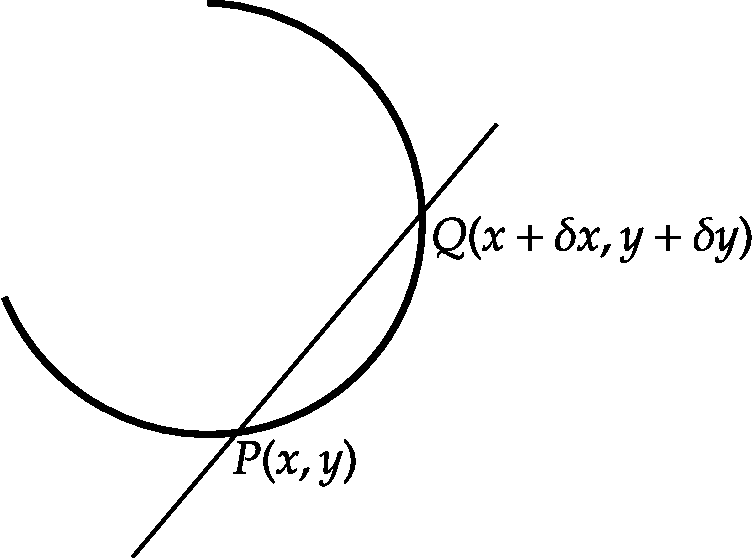
\includegraphics[width=0.25\textwidth]{tangents}
	\end{center}
	\caption{tangent to a curve.}
\end{wrapfigure}
The tangent line to a curve at a given point is the straight line  that touches the curve at that point. The point is called pont of tangency.\\\\
Let $y=f(x)$ be a given curve and $P(x, y)$ and $Q(x+\delta x, y+\delta y)$ be two
neighbouring points on it. Equation of the line $P Q$ is,
\begin{align}
Y-y&=\frac{y+\delta y-y}{x+\delta x-x}(X-x)
\Longrightarrow Y-y=\frac{\delta y}{\delta x}(X-x)
\end{align}
This line will be tangent to the given curve at $P$, if $Q \rightarrow P$ which in turn means that $\delta x \rightarrow 0$ and we know that 

\begin{align}
\lim _{\delta x \rightarrow 0} \frac{\delta y}{\delta x}&=\frac{d y}{d x}\\\text{Therefore the equation of the tangent is,}\notag\\
Y-y&=\frac{d y}{d x}(X-x)
\end{align} 
\subsection{Normals}
The normal at a point $(x, y)$  is the line perpendicular (at right angles) to the tangent at that point. It's slope is given by,
\begin{align}
\text{Slope  }&=\frac{-1}{{d y}/{d x}}\\
\text{And hence equation of the normal is ,}\notag\\
Y-y&=\frac{-1}{d y / d x}(X-x)
\end{align} 

\subsubsection{Geometrical meaning }
$d y / d x$ represents the slope of the tangent to the given curve $y=f(x)$ at any point $(x, y).$
$$ \frac{d y}{d x}=\tan \theta$$($\theta$={The angle which the tangent to the curve makes with +ve direction of $x$ -axis.} )
\section{Monotonic Functions}
  A monotonic function is a function which is either entirely nonincreasing or nondecreasing on an interval $\left( a,b\right) $. A function is monotonic if its first derivative (which need not be continuous) does not change sign.
  \begin{enumerate}
  	\item A function  $f(x)$ is called monotonically increasing (also increasing or non-decreasing) on an interval $\left( a,b\right) $, if,
  	$$ x_{1}\leq x_{2} \Rightarrow  f\left( x_{1}\right) \leq f\left( x_{2}\right) \ \text{For all values of }  x_{1}, x_{2} \in \left( a,b\right)    $$
  	And if,
  	 $$ x_{1} < x_{2} \Rightarrow  f\left( x_{1}\right) < f\left( x_{2}\right) \ \text{For all values of }  x_{1}, x_{2} \in \left( a,b\right)    $$
  	\item 
  	A function $f(x)$ is said to be  decreasing on an interval $\left( a,b\right) $  if, 
  	$$ x_{1}\leq x_{2} \Rightarrow  f\left( x_{1}\right) \geq f\left( x_{2}\right) \ \text{For all values of }  x_{1}, x_{2} \in \left( a,b\right)    $$
  	 A function $f(x)$ is said to be strictly decreasing on an interval $\left( a,b\right) $  if,
  	 	$$ x_{1}< x_{2} \Rightarrow  f\left( x_{1}\right) > f\left( x_{2}\right) \ \text{For all values of }  x_{1}, x_{2} \in \left( a,b\right)    $$
  \end{enumerate}

 \subsubsection{Conditions for Increasing and Decreasing Functions}
 Consider $f(x)$ to be continous on  $ \left[  a, b\right]$ and differentiable on $\left(a,b \right) $ then,
 \begin{itemize}
 \item  If $f^{\prime}(x)>0$ for each $x$ in $(a, b)$ then $f$ is (strictly) increasing on $(a, b)$.
 \item  If $f^{\prime}(x)<0$ for each $x$ in $(a, b)$ then $f$ is (strictly) decreasing on $(a, b)$.
 \item  If $f^{\prime}(x)=0$ for each $x$ in $(a, b)$ then $f$ is a constant function on $(a, b)$.
 \begin{itemize}
 	\item  If $f^{\prime}\left(x^{+}\right)>0$ and $f^{\prime}\left(x^{-}\right)>0$, then increasing at $x$ for all $ x \in (a, b) $.
 	\item If $f^{\prime}\left(x^{+}\right)<0$ and $f^{\prime}\left(x^{-}\right)<0$, then decreasing at $x$ for all $ x \in (a, b) $.
 	\item Otherwise neither increasing nor decreasing.
 \end{itemize}
 \item  If $f^{\prime}(x)=g^{\prime}(x)$ for each $x$ in $(a, b)$ then there exists a constant $c$ such that $f(x)=g(x)+c$ for each $x$ in $(a, b)$.	
 \end{itemize}
\begin{minipage}{0.45\textwidth}
	\begin{figure}[H]
		\centering
		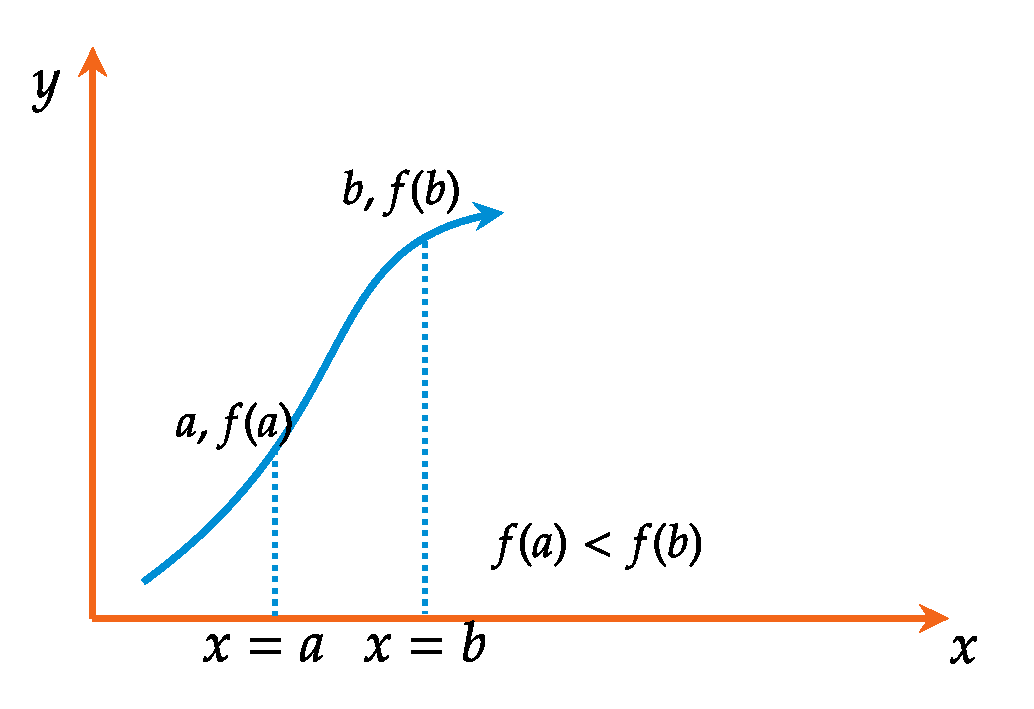
\includegraphics[height=5cm,width=6cm]{increasing}
		\caption{Increasing Function}
		\label{Increasing Function}
	\end{figure}
\end{minipage}
 \begin{minipage}{0.45\textwidth}
 	\begin{figure}[H]
 		\centering
 		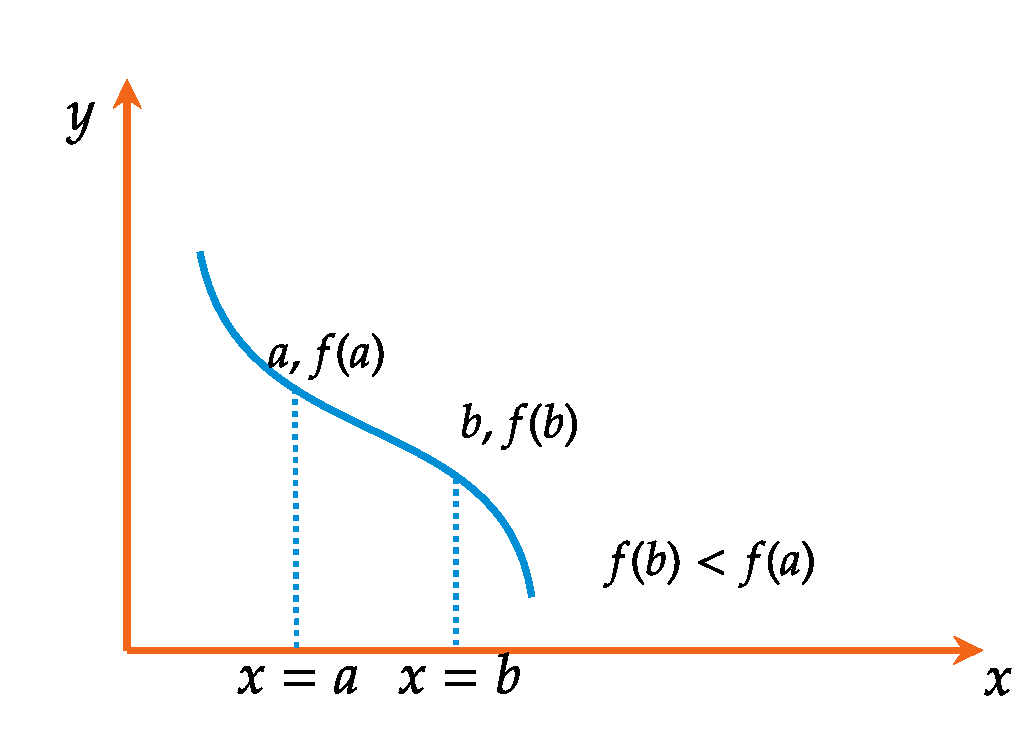
\includegraphics[height=5cm,width=6cm]{decreasing}
 		\caption{Decreasing Function}
 		\label{Decreasing Function}
 	\end{figure}
 \end{minipage}
\begin{exercise}
	Let $f(x)=x^{3}-3 x^{2}+3 x+y .$ Examine the nature of function at $x=0$ and 1 .
\end{exercise}
\begin{answer}
	\begin{align*}
	f(x)&=x^{3}-3 x^{2}+3 x+4 \\ f^{\prime}(x)&=3 x^{2}-6 x+3\\
	\text{At} \quad x&=0,\ f^{\prime}(0)=3>0. \intertext{Hence $f(x)$ is increasing at $x=0$}
	\text{	At } \quad x&=1, f^{\prime}(1)=3-6+3=0 . \intertext{Hence, let's check $f^{\prime}\left(1^{+}\right)$ and $f\left(1^{-}\right)$}
	\text{Clearly,} \quad  f^{\prime}\left(1^{+}\right)&=f(x=1.001)>0\\ \text{And,}\ \left.f^{\prime}(1^{-}\right)&=f(x=0.999)>0
	\intertext{Hence $f(x)$ is increasing at $x=1$.}
\end{align*}
\end{answer}
\section{Maxima and Minima of Functions}
For a continuous and differentiable function $f(x)$ a stationary point $x^{*}$ is a point at which the slope of the function vanishes, i.e. $f^{\prime}(x)=0$ at $x=x^{*}$, where $x^{*}$ belongs to its domain of
definition. A stationary point may be a minimum, maximum or a saddle point(inflection point). 
\subsection{maximum value}
A function $f(x, y)$ is said to have a maximum value at $x=a, y=b$, if there exists a small neighbourhood of $(a, b)$ such that,
$$
f(a, b)>f(a+h, b+k)\ \text{for all values of}\ \left(h,k \right)
$$
\subsection{Minimum value }
A function $f(x, y)$ is said to have a minimum value for $x=a, y=b$, if there exists a small neighbourhood of
 $(a, b)$ such that $$f(a, b)<f(a+h, b+k) \text{for all values of}\ \left(h,k \right)$$.
 \\The maximum and minimum values of a function are also called extreme or extremum values of the function.

 \begin{note}
 	 \leavevmode
 	\\\\
 	\textbf{Saddle point:} It is a point where function is neither maximum nor minimum.
 \end{note}
If $f(a+h, b+k)-f(a, b)$ remains of the same sign for all values (positive or negative) of $(h, k)$, then $f(a, b)$ is said to be extremum value of $f(x, y)$ at $(a, b).$
\begin{itemize}
	\item If $f(a+h, b+k)-f(a, b)<0$, Then $f(a, b)$ is maximum.
	\item If $f(a+h, b+k)-f(a, b)>0$, Then $f(a, b)$ is minimum.
\end{itemize}
\subsubsection{Rules to find Extremum values}
\begin{enumerate}
	\item Differentiate $y=f(x)$ and find out
$\frac{dy}{dx}$
	\item Put $\frac{d y}{d x}=0$ and solve these equations for $x$  . Let one root of $\frac{d y}{d x}=0$ is at $x=a$.
	\item If $\frac{d^{2} y}{d^{2} x}=-v e$ for $x=a$, then maxima is at $x=a$.
	\item If $\frac{d^{2} y}{d^{2} x}=+v e$ for $x=a$, then minima is at $x=a$.
	\item If $\frac{d^{2} y}{d^{2} x}=0$ at $x=a$, then find $\frac{d^{3} y}{d^{3} x}$.
	\\\\If $\frac{d^{3} y}{d^{3} x} \neq 0$ at $x=a$, neither maximum nor minimum at $x=a$.
	\\\\If $\frac{d^{3} y}{d^{3} x}=0$ at $x=a$, then find $\frac{d^{4} y}{d^{4} x}$ and investigate further.
	
\end{enumerate}
\begin{figure}[H]
	\begin{center}
		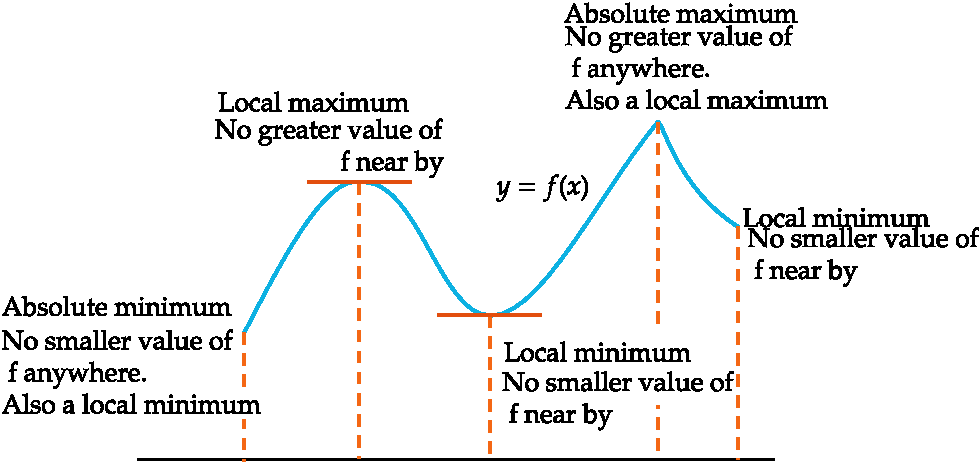
\includegraphics[width=0.75\textwidth]{minima}
	\end{center}
\caption{Minima and Maxima of functions}
\end{figure}
\begin{exercise}
	Find the equilibrium points and  find it's nature.
	\\1.$ f(x)=x^{3}-3x+9$
	\\2.$f(x)=2 x^{3}-21 x^{2}+36 x $
\end{exercise}
\begin{answer}1.
	\begin{align*}
	f^{\prime}(x)&=\frac{df}{dx}=3x^{2}-3\\
	\text{Equating }\quad\frac{df}{dx} &=0\\
	\text{we get,}x&=1,-1\\
	\frac{d^{2}f}{dx^{2}}&=6x\\
	\frac{d^{2}f}{dx^{2}}\bigg\rvert_{x=1}&=6>0\quad(\text{Local minima})\\
	\frac{d^{2}f}{dx^{2}}\bigg\rvert_{x=1}&=-6<0\quad(\text{Local maxima})\\
	\end{align*}
	2.
	\begin{align*}
	 f^{\prime}(x)&=6 x^{2}-42 x+36\\
	 \text{Equating }\quad\frac{df}{dx} &=0\\
	  6 x^{2}-42 x+36&= 0\\
	  (x-1)(x-6)&=0 \rightarrow x=1,6 \\
	  \frac{d^{2}f}{dx^{2}}&=12 x-42\\
	  \frac{d^{2}f}{dx^{2}}\bigg\rvert_{x=1}&=-30<0\quad(\text{Local maxima.})\\
	  \frac{d^{2}f}{dx^{2}}\bigg\rvert_{x=1}&=30>0\quad(\text{Local minima.})
	  \end{align*}
	
\end{answer}

\section{Differentiation}
Let $y=f(x)$ be a differentiable function. The differential $d x$ is an independent variable.Then the differential $d y$ is given by,
\begin{align*}
d y&=f^{\prime}(x) d x\\
\frac{d y}{d x}&=f^{\prime}(x)
\end{align*}
\subsection{Important Properties of Differentiation} 
\begin{enumerate}
	\item $\frac{d}{d x}(f(x)+g(x))=\frac{d}{d x} f(x)+\frac{d}{d x} g(x)$
	\item $\frac{d}{d x}(f(x)-g(x))=\frac{d}{d x} f(x)-\frac{d}{d x} g(x)$
	\item $\frac{d}{d x}(f(x) \cdot g(x))=f(x) \cdot \frac{d}{d x}(g(x))+\frac{d}{d x}(f(x)) \cdot g(x)$
	\item $\frac{d}{d x}\left(\frac{f(x)}{g(x)}\right)=\frac{\frac{d}{d x} f(x) \cdot g(x)-f(x) \frac{d}{d x} g(x)}{(g(x))^{2}}$
\end{enumerate}
\textcolor{ocre}{(\large * The section \ref{partial diferentiation} can be omitted without losing continuity.)}
\subsection{Partial Differentiation}\label{partial diferentiation}
\begin{definition}
	The partial derivative of $\boldsymbol{f}(\boldsymbol{x}, \boldsymbol{y})$ with respect to $\boldsymbol{y}$ at the point $\left(x_{0}, y_{0}\right)$ is
	$$
	\left.\frac{\partial f}{\partial y}\right|_{\left(x_{0}, y_{0}\right)}=\left.\frac{d}{d y} f\left(x_{0}, y\right)\right|_{y=y_{0}}=\lim _{h \rightarrow 0} \frac{f\left(x_{0}, y_{0}+h\right)-f\left(x_{0}, y_{0}\right)}{h},
	$$
	provided the limit exists.
\end{definition}
If a derivative of function of several independent variable, $f(x,y,z..)$ be found with respect to any one of them, keeping the others as constants, it is said to be partial derivative .And the operation of finding is called partial differentiation.
\\\\The partial derivative of $f(x, y)$ with respect to $x$ and $y$ are generally denoted by,
\begin{align*}f_{x}=\frac{\partial f}{\partial x}\quad &;\quad f_{y}=\frac{\partial f}{\partial y}\\
 \frac{\partial}{\partial x}\left(\frac{\partial f}{\partial x}\right) \equiv \frac{\partial^{2} f}{\partial x^{2}} \equiv f_{x x}\quad &;\quad \frac{\partial}{\partial y}\left(\frac{\partial f}{\partial y}\right) \equiv \frac{\partial^{2} f}{\partial y^{2}} \equiv f_{y y} \\
	\frac{\partial}{\partial x}\left(\frac{\partial f}{\partial y}\right) \equiv \frac{\partial^{2} f}{\partial x \partial y} \equiv f_{x y} \quad &;\quad \frac{\partial}{\partial y}\left(\frac{\partial f}{\partial x}\right) \equiv \frac{\partial^{2} f}{\partial y \partial x} \equiv f_{y x}\quad \text { it is given that } f_{x y}=f_{y x}
\end{align*}
\begin{exercise}
	Find $\partial f / \partial y$ if $f(x, y)=y \sin x y$.
	
\end{exercise}
\begin{answer}
We treat $x$ as a constant and $f$ as a product of $y$ and $\sin x y$ :
\begin{align*}
\frac{\partial f}{\partial y} &=\frac{\partial}{\partial y}(y \sin x y)=y \frac{\partial}{\partial y} \sin x y+(\sin x y) \frac{\partial}{\partial y}(y) \\
&=(y \cos x y) \frac{\partial}{\partial y}(x y)+\sin x y\\&=x y \cos x y+\sin x y .
\end{align*}
\end{answer}
\begin{exercise}
	Find the values of $\partial f / \partial x$ and $\partial f / \partial y$ at the point $(4,-5)$ if
	$f(x, y)=x^{2}+3 x y+y-1$
\end{exercise}
\begin{answer}
	 To find $\partial f / \partial x$, we treat $y$ as a constant and differentiate with respect to $x$
	 \begin{align*}
	 \frac{\partial f}{\partial x}&=\frac{\partial}{\partial x}\left(x^{2}+3 x y+y-1\right)\\&=2 x+3 \cdot 1 \cdot y+0-0=2 x+3 y\\
	 \partial f / \partial x|_{(4,5)} &=
	 	(4)+3(-5)=-7
	 \end{align*}
To find $\partial f / \partial y$, we treat $x$ as a constant and differentiate with respect to $y$ :
	\begin{align*}
\frac{\partial f}{\partial y}&=\frac{\partial}{\partial y}\left(x^{2}+3 x y+y-1\right)=0+3 \cdot x \cdot 1+1-0=3 x+1\\
\partial f / \partial y|_{(4,5)}&= 3(4)+1=13
	\end{align*}
	
\end{answer}
\begin{theorem}
	\textbf{Euler's theorem:} \\If $u$ is a homogenous function of degree ' $n$ ' in $x$ and $y$ then
	$$
	x \frac{\partial u}{\partial x}+y \frac{\partial u}{\partial y}=n u
	$$
	For any number of variables,
	$$
	x \frac{\partial u}{\partial x}+y \frac{\partial u}{\partial y}+z \frac{\partial u}{\partial z}+\ldots \ldots \ldots+w \frac{\partial u}{\partial w}=n u
	$$
\end{theorem}
\begin{note}
	\begin{align*}
		&\text{If, }u=f(x, y) \text{but, } \quad x=\phi(s, t); \quad y=\phi(s, t);\\
		\text{Then, }&\frac{\partial u}{\partial s}=\frac{\partial u}{\partial x} \cdot \frac{\partial x}{\partial s}+\frac{\partial u}{\partial y} \cdot \frac{\partial y}{\partial s}\quad \text { and }\quad \frac{\partial u}{\partial t}=\frac{\partial u}{\partial x} \cdot \frac{\partial x}{\partial t}+\frac{\partial u}{\partial y} \cdot \frac{\partial y}{\partial t}
	\end{align*}
\end{note}
\begin{exercise}
	Find $\partial z / \partial x$ if the equation
	$$
	y z-\ln z=x+y
	$$
	defines $z$ as a function of the two independent variables $x$ and $y$ and the partial derivative exists.
\end{exercise}
\begin{answer}
	We differentiate both sides of the equation with respect to $x$, holding $y$ constant and treating $z$ as a differentiable function of $x$ :
	\begin{align*}
		\frac{\partial}{\partial x}(y z)-\frac{\partial}{\partial x} \ln z &=\frac{\partial x}{\partial x}+\frac{\partial y}{\partial x} \\
		y \frac{\partial z}{\partial x}-\frac{1}{z} \frac{\partial z}{\partial x} &=1+0 \hspace{4cm}
		 \begin{array}{l}
			\text { With } y \text { constant, } \\
			\frac{\partial}{\partial x}(y z)=y \frac{\partial z}{\partial x}
		\end{array} \\
		\left(y-\frac{1}{z}\right) \frac{\partial z}{\partial x}&=1 \\
		\frac{\partial z}{\partial x}&=\frac{z}{y z-1}
	\end{align*}
\end{answer}
\section{Integration}
\subsection{Definite and Indefinite Integrals}
\subsection{Definite Integrals}
If a function $f(x)$ is defined in the interval $[a, b]$, then the definite integral of the function is given by
$$
\int_{a}^{b} f(x) \cdot d x=[F(x)]_{a}^{b}=F(b)-F(a)
$$
Where $F(x)$ is an integral of $f(x), a$ is called the lower limit and $b$ is the upper limit of the integral.
Geometrically, a definite integral represents the area bounded by a curve, $y=f(x), x$ -axis and the lines $x=a$ and $x=b$.
\subsubsection{Properties}
\begin{enumerate}
	\item $ \int_{a}^{b} f(x) \cdot d x=\int_{a}^{b} f(y) \cdot d y$
	\item  $\int_{a}^{b} f(x) \cdot d x=-\int_{b}^{a} f(x) \cdot d x$
	\item  $\int_{a}^{b} f(x) \cdot d x=\int_{a}^{c} f(x) \cdot d x+\int_{c}^{b} f(x) \cdot d x \quad$ if $a<c<b$
	\item $\int_{0}^{2 a} f(x) \cdot d x=\int_{0}^{a} f(x) \cdot d x+\int_{0}^{a} f(2 a-x) \cdot d x$
	\item $\int_{0}^{a} f(x) \cdot d x=\int_{0}^{a} f(a-x) \cdot d x$
	\item $\int_{-a}^{a} f(x) \cdot d x=2 \int_{0}^{a} f(x) \cdot d x$, If the function is even. $\int_{-a}^{a} f(x) \cdot d x=0$, if the function is odd.
	\item $\int_{0}^{n a} f(x) \cdot d x=n \int_{0}^{a} f(x) \cdot d x$ if $f(x)=f(x+a)$
\end{enumerate}
\subsection{Indefinite Integrals}
The set of all antiderivatives of the function $ f$ is called the
indefinite integral of $ f$ with respect to $ x$, and is symbolized by,
$$
\int f(x) d x
$$
An indefinite integral $\int f(x) d x$ is a function plus an arbitrary constant $C$.
\subsection{Methods of Integration}

\subsection{Integration by Substitution}
If $u=g(x)$ is a differentiable function whose range is an interval $I$ and $f$ is continuous on $I$, then
$$
\int f(g(x)) g^{\prime}(x) d x=\int f(u) d u
$$
\textbf{ Method of solving}
\begin{enumerate}
	\item Substitute $u=g(x)$ and $d u=g^{\prime}(x) d x$ to obtain the integral
	$$
	\int f(u) d u
	$$
	\item Integrate with respect to $u$.
	\item Replace $u$ by $g(x)$ in the result.
\end{enumerate}

\begin{exercise}
	Integrate 
	\begin{enumerate}
		\item $\int x^{2} \sin \left(x^{3}\right) d x$
		\item $ \int \frac{1}{\cos ^{2} 2 x} d x$
		\item $ \int \sin ^{2} x d x$
	\end{enumerate}
\end{exercise}
\begin{answer}1.\hspace{0.5cm}
	
\begin{minipage}{0.45\textwidth}
	\begin{align*}
	\int x^{2} \sin \left(x^{3}\right) d x &=\int \sin \left(x^{3}\right) \cdot x^{2} d x \\
	&=\int \sin u \cdot \frac{1}{3} d u \\
	&=\frac{1}{3} \int \sin u d u \\
	&=\frac{1}{3}(-\cos u)+C \\
	&=-\frac{1}{3} \cos \left(x^{3}\right)+C
	\end{align*}
\end{minipage}\hspace{2.5cm}
\begin{minipage}{0.35\textwidth}\hfill
		
	\begin{align*}
	&\text{Let,}u=x^{3}\\
	&d u=3 x^{2} d x \\
	&(1 / 3) d u=x^{2} d x\\
	&\text{Integrate}\text{ with respect to $u$}\\\\\\
	&\text{Replace $u$ by $x^{3}$.}
	\end{align*}
\end{minipage}
	

	\begin{minipage}{0.45\textwidth}
		2.\vspace{0.2cm}
		\begin{align*}
		\int \frac{1}{\cos ^{2} 2 x} d x &=\int \sec ^{2} 2 x d x \\
		&=\int \sec ^{2} u \cdot \frac{1}{2} d u \\
		&=\frac{1}{2} \int \sec ^{2} u d u \\
		&=\frac{1}{2} \tan u+C \\
		&=\frac{1}{2} \tan 2 x+C
		\end{align*}
	\end{minipage}\hspace{2.5cm}
\begin{minipage}{0.35\textwidth}\hfill
	
	\begin{align*}
	&\frac{1}{\cos 2 x}=\sec 2 x \\
	&u=2 x \\
	&d u=2 d x \\
	&d x=(1 / 2) d u \\
	\\
	&\frac{d}{d u} \tan u=\sec ^{2} u \\
	&u=2 x
\end{align*}
\end{minipage}\\\\
3.\vspace{0.2cm}\begin{align*}
\int \sin ^{2} x d x &=\int \frac{1-\cos 2 x}{2} d x \quad \sin ^{2} x=\frac{1-\cos 2 x}{2}\hspace{2cm} \because\sin ^{2} x=\frac{1-\cos 2 x}{2}\\
&=\frac{1}{2} \int(1-\cos 2 x) d x=\frac{1}{2} \int d x-\frac{1}{2} \int \cos 2 x d x \\
&=\frac{1}{2} x-\frac{1}{2} \frac{\sin 2 x}{2}+C=\frac{x}{2}-\frac{\sin 2 x}{4}+C
\end{align*}
\end{answer}
\subsection{Integration by Parts}
Integration by parts is a technique for performing integration (definite and indefinite) by expanding the differential of a product of function $d(u v)$ and expressing the original integral in terms of a known integral.
$$ \int f(x) g^{\prime}(x) d x=f(x) g(x)-\int f^{\prime}(x) g(x) d x$$
 Let $u=f(x)$ and $v=g(x)$. Then $d u=f^{\prime}(x) d x$ and $d v=g^{\prime}(x) d x$.
Then,
\begin{center}
	\framebox{
		
		\parbox[t][1cm]{4cm}{
			
			\addvspace{0.3cm} \centering 
			$\int u d v=u v-\int v d u$	} 	}
\end{center}
\begin{note}\leavevmode \newline
For definite integral, $\left.\int_{a}^{b} f(x) g^{\prime}(x) d x=f(x) g(x)\right]_{a}^{b}-\int_{a}^{b} f^{\prime}(x) g(x) d x$
\end{note}
\subsubsection{Tabular Integration}
\begin{minipage}{0.5\textwidth}
Tabular integration is a special technique for integration by parts. It can be applied to certain functions in the form $f(x)g(x)$, where one of $f(x)$ or $g(x)$  can be differentiated multiple times with ease, while the other function can be integrated multiple times with ease.
\end{minipage}
\begin{minipage}{0.5\textwidth}

\begin{figure}[H]
		\centering
	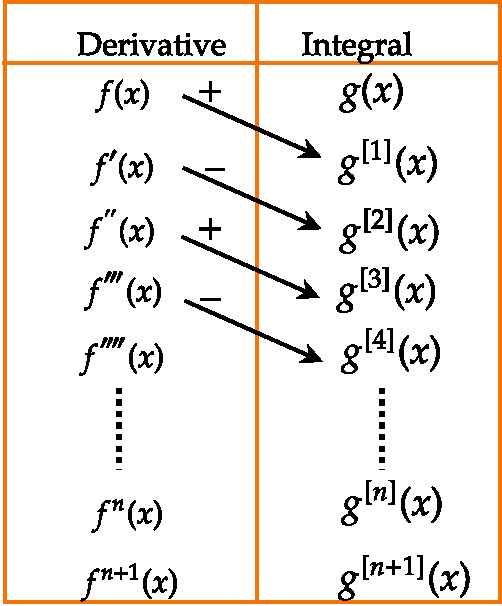
\includegraphics[width=5cm, height=5cm]{tabular integration}
	\caption{Tabular integration}
\end{figure}
\end{minipage}

\textbf{Method of solving}
\begin{enumerate}
	\item In the product comprising the function , identify the polynomial and denote it $f(x)$. Denote the other function in the product by $g(x)$.
	\item Create a table of $f(x)$ and $g(x)$, and successively differentiate $f(x)$ until you reach 0 . Successively integrate $g(x)$ the same amount of times.
	\item Construct the integral by taking the product of $f(x)$ and the first integral of $g(x)$, then add the product of $f^{\prime}(x)$ times the second integral of $g(x)$, then add the product of $f^{\prime \prime}(x)$ times the third integral of $g(x)$, etc...
\end{enumerate}

{\begin{exercise}
		Integrate $\int x^{2} e^{x} d x$
	\end{exercise}
	
	\begin{answer}.\\
		\begin{minipage}{0.45\textwidth}
			\begin{align*}
			\text { With } f(x)=x^{2} \text { and } g(x)&=e^{x} \text { , we list: }\\
			\end{align*}
			We combine the products of the functions connected by the arrows according to the operation signs above the arrows to obtain	
			\begin{align*}
			\int x^{2} e^{x} d x&=x^{2} e^{x}-2 x e^{x}+2 e^{x}+C
			\end{align*}
			
			
		\end{minipage}\hspace{2.5cm}
		\begin{minipage}{0.35\textwidth}\hfill
			
			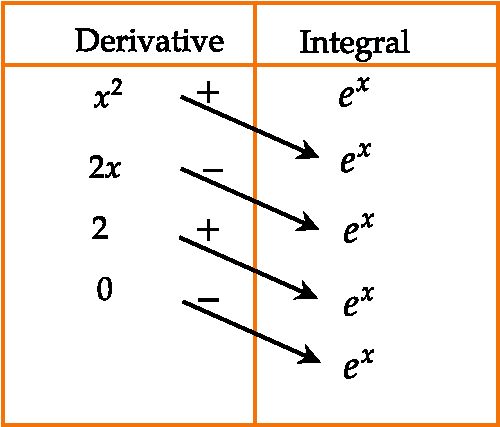
\includegraphics[width=0.65\textwidth]{tabularex}
		\end{minipage}
\end{answer}}


\subsection{Integration by Partial fraction}
The method of integrating rational functions (of the form\quad$\frac{P(x)}{Q(x)}$)\quad as a sum of simpler fractions is called the method of partial fraction.This method  works by algebraically splitting $P(x) / Q(x)$ into pieces that are easier to integrate.
\subsubsection{Method of solving}
\begin{enumerate}
	\item Let $x-r$ be a linear factor of $Q(x)$. Suppose that $(x-r)^{m}$ is the highest power of $x-r$ that divides $Q(x)$. Then, to this factor, assign the sum of the $m$ partial fractions:
	$$
	\frac{A_{1}}{x-r}+\frac{A_{2}}{(x-r)^{2}}+\cdots+\frac{A_{m}}{(x-r)^{m}}
	$$
	Do this for each distinct linear factor of $Q(x)$
	\item Let $x^{2}+p x+q$ be a quadratic factor of $Q(x)$. Suppose that $\left(x^{2}+p x+q\right)^{n}$ is the highest power of this factor that divides $Q(x)$. Then, to this factor, assign the sum of the $n$ partial fractions:
	$$
	\frac{B_{1} x+C_{1}}{x^{2}+p x+q}+\frac{B_{2} x+C_{2}}{\left(x^{2}+p x+q\right)^{2}}+\cdots+\frac{B_{n} x+C_{n}}{\left(x^{2}+p x+q\right)^{n}}
	$$
	Do this for each distinct quadratic factor of $Q(x)$ that cannot be factored into linear factors with real coefficients.
	\item Set the original fraction $P(x) / Q(x)$ equal to the sum of all these partial fractions. Clear the resulting equation of fractions and arrange the terms in decreasing powers of $x$.
	\item Equate the coefficients of corresponding powers of $x$ and solve the resulting equations for the undetermined coefficients.
\end{enumerate}
\begin{exercise}
	Integrate $
	\int \frac{6 x+7}{(x+2)^{2}} d x
	$
\end{exercise}
\begin{answer}
	Express the integrand as a sum of partial fractions with undetermined coefficients.
	\begin{align*}
	\frac{6 x+7}{(x+2)^{2}}&=\frac{A}{x+2}+\frac{B}{(x+2)^{2}}\qquad(\rightarrow\text{Multiply both sides by} (x+2)^{2})\\
	6 x+7 &=A(x+2)+B \\
	&=A x+(2 A+B)
	\end{align*}
	{Equating coefficients of corresponding powers of $x$ gives}
	\begin{align*}
	A=6 \quad \text{and} \quad 2 A+B=12+B=7, &\quad \text{or} \quad A=6 \quad \text{and} \quad B=-5.\\
	\therefore \int \frac{6 x+7}{(x+2)^{2}} d x &=\int\left(\frac{6}{x+2}-\frac{5}{(x+2)^{2}}\right) d x \\
	&=6 \int \frac{d x}{x+2}-5 \int(x+2)^{-2} d x \\
	&=6 \ln |x+2|+5(x+2)^{-1}+C
	\end{align*}
\end{answer}
\begin{exercise}
	Integrate $\int \frac{2 x^{3}-4 x^{2}-x-3}{x^{2}-2 x-3} d x$
\end{exercise}
\newcommand{\longdiv}{\smash{\mkern-0.43mu\vstretch{1.31}{\hstretch{.7}{)}}\mkern-5.2mu\vstretch{1.31}{\hstretch{.7}{)}}}}
\begin{answer}The given function is an improper fraction.First we need to divide the denominator into the numerator to get a polynomial plus a proper fraction.
	
	\[
	\arraycolsep=0.5pt
	\renewcommand\arraystretch{0.6}
	\begin{array}{*1r @{\hskip\arraycolsep}c@{\hskip\arraycolsep} *{11}r}
	&          & 2x &  &  & &  &  &  &  &  &  &   \\
	\cline{2-13}
	x ^ { 2 } - 2 x - 3  &\longdiv &  2 x ^ { 3 } & -  & 4 x ^ { 2 }   & -  &  x     & -  & 3     &   &      &   &        \\
	&          & 2 x ^ { 3 } & - & 4 x ^ { 2 } & - &  6x &   &      &   &      &   &        \\
	\cline{3-7}
	&          &   &   &  &  &   & 5x  & -     & 3  &      &   &        
	\end{array}
	\]
	Then we write the improper fraction as a polynomial plus a proper fraction.
	\begin{align*}
	\frac{2 x^{3}-4 x^{2}-x-3}{x^{2}-2 x-3}&=2 x+\frac{5 x-3}{x^{2}-2 x-3}\\
	\text{and then,}\\
	\int \frac{2 x^{3}-4 x^{2}-x-3}{x^{2}-2 x-3} d x &=\int 2 x d x+\int \frac{5 x-3}{x^{2}-2 x-3} d x \\
	&=\int 2 x d x+\int \frac{2}{x+1} d x+\int \frac{3}{x-3} d x \\
	&=x^{2}+2 \ln |x+1|+3 \ln |x-3|+C
	\end{align*}
	
	
\end{answer}
\subsection{Trigonometrtic Integrals}
Trigonometric integrals involve algebraic combinations of the six basic trigonometric
functions.
\subsubsection{Trigonmetric Substitution}
Trigonometric substitution is used to simplify certain integrals containing radical expressions. Depending on the function we need to integrate, we substitute one of the following expressions:
\begin{itemize}
	\item For $\sqrt{a^{2}-x^{2}}$, use $x=a \sin \theta$.
	\item For $\sqrt{a^{2}+x^{2}}$, use $x=a \tan \theta$.
	\item For $\sqrt{x^{2}-a^{2}}$, use $x=a \sec \theta$.
\end{itemize}
\subsubsection{Powers of sines and cosines}
For the integrals of the form $$\int \sin ^{m} x \cos ^{n} x d x$$
\begin{itemize}
	\item If , \textbf{m=n=odd}\\
	Write $m$ as $2 k+1$ and use the identity $\sin ^{2} x=1-\cos ^{2} x$ to obtain
	$$
	\sin ^{m} x=\sin ^{2 k+1} x=\left(\sin ^{2} x\right)^{k} \sin x=\left(1-\cos ^{2} x\right)^{k} \sin x
	$$
	Then combine the single $\sin x$ with $d x$ in the integral and set $\sin x d x$ equal to $-d(\cos x)$.
	\item If , \textbf{m=even and n=odd}\\
	 Write $n$ as $2 k+1$ and use the identity $\cos ^{2} x=1-\sin ^{2} x$ to obtain
	$$
	\cos ^{n} x=\cos ^{2 k+1} x=\left(\cos ^{2} x\right)^{k} \cos x=\left(1-\sin ^{2} x\right)^{k} \cos x .
	$$
	Then combine the single $\cos x$ with $d x$ and set $\cos x d x$ equal to $d(\sin x)$.
	\item If , \textbf{m=n=even}\\
	Substitute
	$$
	\sin ^{2} x=\frac{1-\cos 2 x}{2}, \quad \cos ^{2} x=\frac{1+\cos 2 x}{2}
	$$
	To reduce the integrand to one in lower powers of $\cos 2 x$.
\end{itemize}

\begin{note}\newline
	$\begin{array}{l}
		\sin m x \sin n x=\frac{1}{2}[\cos (m-n) x-\cos (m+n) x] \\\\
		\sin m x \cos n x=\frac{1}{2}[\sin (m-n) x+\sin (m+n) x] \\\\
		\cos m x \cos n x=\frac{1}{2}[\cos (m-n) x+\cos (m+n) x]
	\end{array}$
\end{note}
\begin{exercise}
	Evaluate $\int \cos ^{5} x d x$
\end{exercise}
\begin{answer}
	\begin{align*} 
	\int \cos ^{5} x d x &=\int \cos ^{4} x \cos x d x=\int\left(1-\sin ^{2} x\right)^{2} d(\sin x) \\ &=\int\left(1-u^{2}\right)^{2} d u \\ &=\int\left(1-2 u^{2}+u^{4}\right) d u \\ &=u-\frac{2}{3} u^{3}+\frac{1}{5} u^{5}+C=\sin x-\frac{2}{3} \sin ^{3} x+\frac{1}{5} \sin ^{5} x+C 
	\end{align*}
\end{answer}
\begin{exercise}
	Evaluate $\int_{0}^{\pi / 4} \sqrt{1+\cos 4 x} d x$
\end{exercise}
\begin{answer}
 $\quad$ To eliminate the square root we use the identity
	$$
	\cos ^{2} \theta=\frac{1+\cos 2 \theta}{2}, \quad \text { or } \quad 1+\cos 2 \theta=2 \cos ^{2} \theta
	$$
\begin{align*}
		\intertext{With $\theta=2 x$, this becomes}
	1+\cos 4 x&=2 \cos ^{2} 2 x\\
	\int_{0}^{\pi / 4} \sqrt{1+\cos 4 x} d x &=\int_{0}^{\pi / 4} \sqrt{2 \cos ^{2} 2 x} d x=\int_{0}^{\pi / 4} \sqrt{2} \sqrt{\cos ^{2} 2 x} d x \\
		&=\sqrt{2} \int_{0}^{\pi / 4}|\cos 2 x| d x=\sqrt{2} \int_{0}^{\pi / 4} \cos 2 x d x \quad \begin{array}{l}
			\cos 2 x \geq 0 \\
			\text { on }[0, \pi / 4]
		\end{array} \\
		&=\sqrt{2}\left[\frac{\sin 2 x}{2}\right]_{0}^{\pi / 4}=\frac{\sqrt{2}}{2}[1-0]=\frac{\sqrt{2}}{2}
	\end{align*}
\end{answer}
\begin{exercise}
 Evaluate,	$\int \frac{x^{2} d x}{\sqrt{9-x^{2}}}$
\end{exercise}
\begin{answer}
		\begin{alignat*}{2}
		\text{Let, }&x=3 \sin \theta, \quad d x=3 \cos \theta d \theta, &&\quad-\frac{\pi}{2}<\theta<\frac{\pi}{2} \\
		&9-x^{2}=9-9 \sin ^{2} \theta=9\left(1-\sin ^{2} \theta\right)&&=9 \cos ^{2} \theta\\
	\end{alignat*}
	Then
	\begin{align*}
	\int \frac{x^{2} d x}{\sqrt{9-x^{2}}} &=\int \frac{9 \sin ^{2} \theta \cdot 3 \cos \theta d \theta}{|3 \cos \theta|} \\
	&=9 \int \sin ^{2} \theta d \theta \quad \cos \theta>0 \text { for }-\frac{\pi}{2}<\theta<\frac{\pi}{2} \\
	&=9 \int \frac{1-\cos 2 \theta}{2} d \theta \\
	&=\frac{9}{2}\left(\theta-\frac{\sin 2 \theta}{2}\right)+C \qquad |\sin 2 \theta=2 \sin \theta \cos \theta \\
	&=\frac{9}{2}(\theta-\sin \theta \cos \theta)+C \quad \\
	&=\frac{9}{2}\left(\sin ^{-1} \frac{x}{3}-\frac{x}{3} \cdot \frac{\sqrt{9-x^{2}}}{3}\right)+C  \\
	&=\frac{9}{2} \sin ^{-1} \frac{x}{3}-\frac{x}{2} \sqrt{9-x^{2}}+C
	\end{align*}
	
\end{answer}
\begin{exercise}
	Evaluate
	$\int \sin 3 x \cos 5 x d x$
\end{exercise}
\begin{answer}
	We know that ,\quad $\sin m x \cos n x=\frac{1}{2}[\sin (m-n) x+\sin (m+n) x]$\\
	\begin{align*}
	\text{m = 3 and n = 5 we get}\\
		\int \sin 3 x \cos 5 x d x &=\frac{1}{2} \int[\sin (-2 x)+\sin 8 x] d x \\
		&=\frac{1}{2} \int(\sin 8 x-\sin 2 x) d x \\
		&=-\frac{\cos 8 x}{16}+\frac{\cos 2 x}{4}+C
	\end{align*}
\end{answer}

\section{Summation and Serises}
\begin{minipage}{0.45\textwidth}
	\begin{center}
		\framebox{
			\parbox[t][5cm]{3cm}{
				
				\addvspace{0.2cm} \centering 
				
				\begin{align*}
			&\text{\textbf{Sum of Arithmatic series}}\\
			S&=\sum_{n=0}^{+N} [a+(n-1)d]\\
			S_{N}&=\frac{N}{2}[a+l] \rightarrow (l= \text{Last term})\\
			S_{N}&=\frac{N}{2}[2a+(n-1)d]
			\end{align*}} }
	\end{center}
\end{minipage}
\begin{minipage}{0.45\textwidth}
	\begin{center}
		\framebox{
			\parbox[t][5cm]{3cm}{
				
				\addvspace{0.2cm} \centering 
				
				\begin{align*}
				&\text{\textbf{Sum of Geometric series}}\\
				&S_{n}=\frac{a(1-r^{n})}{1-r}\qquad (r<1)\\
				&S_{n}=\frac{a(r^{n}-1)}{r-1}\qquad (r>1)\\
				&\text{\textbf{\large Sum of Infinite series}}\\
				&S_{n}=\frac{a}{r-1}
				\end{align*}} }
	\end{center}
\end{minipage}
\section{Binomial Theorem}
\begin{theorem}
	For any positive integer $ n $, the $ n ^{\text{th }}$power of the sum of two numbers $ a $ and $ b $ may be expressed as the sum of $ n + 1 $ terms of the form,
\begin{equation}
		$$(a+b)^{n}= \sum_{n=o}^{r} {^{n}C_{r} a^{n-r}b^{r}}$$
\end{equation}

\end{theorem}
\section{Taylor and Maclaurin series}
\begin{definition}
	Let $f$ be a function with derivatives of all orders throughout some interval containing $a$ as an interior point. Then the Taylor series generated by $f$ at $x=a$ is
	$$
	\begin{aligned}
	\sum_{k=0}^{\infty} \frac{f^{(k)}(a)}{k !}(x-a)^{k}=f(a)+f^{\prime} &(a)(x-a)+\frac{f^{\prime \prime}(a)}{2 !}(x-a)^{2} +\cdots+\frac{f^{(n)}(a)}{n !}(x-a)^{n}+\cdots
	\end{aligned}
	$$
	The Maclaurin series generated by $f$ is
	$$
	\sum_{k=0}^{\infty} \frac{f^{(k)}(0)}{k !} x^{k}=f(0)+f^{\prime}(0) x+\frac{f^{\prime \prime}(0)}{2 !} x^{2}+\cdots+\frac{f^{(n)}(0)}{n !} x^{n}+\cdots,
	$$
	The Taylor series generated by $f$ at $x=0$.
\end{definition}
\subsubsection{Taylor polynomial}
Let $f$ be a function with derivatives of order $k$ for $k=1,2, \ldots, N$ in some interval containing $a$ as an interior point. Then for any integer $n$ from 0 through $N$, the Taylor polynomial of order $n$ generated by $f$ at $x=a$ is the polynomial,
$$
\begin{aligned}
P_{n}(x)=f(a)+f^{\prime}(a)(x-a) &+\frac{f^{\prime \prime}(a)}{2 !}(x-a)^{2}+\cdots \\
&+\frac{f^{(k)}(a)}{k !}(x-a)^{k}+\cdots+\frac{f^{(n)}(a)}{n !}(x-a)^{n} .
\end{aligned}
$$
\begin{exercise}
	Find the Taylor series and the Taylor polynomials generated by $f(x)=e^{x}$ at $x=0$.
\end{exercise}
\begin{answer}
	$$
	f(x)=e^{x}, \quad f^{\prime}(x)=e^{x}, \quad \ldots, \quad f^{(n)}(x)=e^{x}, \quad \ldots
	$$
	we have
	$$
	f(0)=e^{0}=1, \quad f^{\prime}(0)=1, \quad \ldots, \quad f^{(n)}(0)=1, \quad \ldots
	$$
	The Taylor series generated by $f$ at $x=0$ is
	\begin{align*}
	f(0)+f^{\prime}(0) x+\frac{f^{\prime \prime}(0)}{2 !} x^{2}+\cdots &+\frac{f^{(n)}(0)}{n !} x^{n}+\cdots \\
	&=1+x+\frac{x^{2}}{2}+\cdots+\frac{x^{n}}{n !}+\cdots \\
	&=\sum_{k=0}^{\infty} \frac{x^{k}}{k !}
	\end{align*}
	
\end{answer}
\begin{exercise}
	In the Taylor's series expansion of $e^{x}$ about $x=2$, the coefficient of $(x-2)^{4}$ is
\end{exercise}
\begin{answer}
	$f(x)$ in the neighborhood of $a$ is given by
	\begin{align*}
f(x)=\sum_{n=0}^{\infty} b_{n}(x-a)^{n}\\
\text{where} b_{n}&=\frac{f^{n}(a)}{n !}\\
f^{4}(x)&=e^{x} \cdot f^{4}(2)=e^{2}\\
\text{Therefore, coefficient of}(x-2)^{4}&=b_{4}=\frac{f^{4}(2)}{4 !}=\frac{e^{2}}{4 !}
\end{align*}
\end{answer}
\newpage
\colorlet{ocre1}{ocre!70!}
\colorlet{ocrel}{ocre!30!}
\begin{table}[H]
	\centering
	\arrayrulecolor{ocre}
	\renewcommand{\arraystretch}{1.7}
	\begin{tabularx}{0.8\textwidth} { 
			| >{\centering\arraybackslash}X 
			| >{\centering\arraybackslash}X |  }
		\hline
		\rowcolor{ocrel}\large \textbf{Derivatives} & \large \textbf{Integrals} \\
		\hline
		$\frac{d}{d x}\left(\frac{x^{n +1}}{n+1}\right)=x^{n} $ & $\int x^{n} d x=\frac{x^{n+1}}{n+1}+C$   \\
		\hline
		$ \frac{d}{d x}(x)=1 $& $ \int d x=x+C $\\ \hline
		$ \frac{d}{d x}(\sin x)=\cos x$& $\int \cos x d x=\sin x+C $\\ \hline
		$\frac{d}{d x}(-\cos x)=\sin x $& $ \int \sin x d x=-\cos x+C$\\ \hline
		$\frac{d}{d x}(\tan x)=\sec ^{2} x  $& $ \int \sec ^{2} x d x=\tan x+C $\\ \hline
		$ \frac{d}{d x}(-\cot x)=\operatorname{cosec}^{2} x$& $ \int \operatorname{cosec}^{2} x d x=-\cot x+C $\\ \hline
		$ \frac{d}{d x}(\sec x)=\sec x \tan x $& $ \int \sec x \tan x d x=\sec x+C $\\ \hline
		$\frac{d}{d x}(-\operatorname{cosec} x)=\operatorname{cosec} x \cot x $& $\int \operatorname{cosec} x \cot x d x=-\operatorname{cosec} x+C $\\ \hline
		$ \frac{d}{d x}\left(\sin ^{-1} x\right)=\frac{1}{\sqrt{1-x^{2}}} $& $\int \frac{\mathrm{d} x}{\sqrt{1-x^{2}}}=\sin ^{-1} x+C $\\ \hline
		$\frac{d}{d x}\left(\cos ^{-1} x\right)=-\frac{1}{\sqrt{1-x^{2}}}  $& $\int-\frac{d x}{\sqrt{1-x^{2}}}=\cos ^{-1} x+C  $\\ \hline
		$ \frac{d}{d x}\left(\tan ^{-1} x\right)=\frac{1}{1+x^{2}} $& $\int \frac{d x}{1+x^{2}}=\tan ^{-1} x+C $\\ \hline
		$ \frac{d}{d x}\left(\cot ^{-1} x\right)=-\frac{1}{1+x^{2}} $& $\int-\frac{d x}{1+x^{2}}=\cot ^{-1} x+C $\\ \hline
		$\frac{d}{d x}\left(\sec ^{-1} x\right)=\frac{1}{|x| \sqrt{x^{2}-1}}  $& $\int \frac{d x}{|x| \sqrt{x^{2}-1}}=\sec ^{-1} x+C $\\ \hline
		$ \frac{d}{d x}\left(\operatorname{cosec}^{-1} x\right)=-\frac{1}{|x| \sqrt{x^{2}-1}}$& $\int \frac{d x}{-|x| \sqrt{x^{2}-1}}=\operatorname{cosec}^{-1} x+C  $\\ \hline
		$ \frac{d}{d x}\left(e^{x}\right)=e^{x} $& $ \int e^{x} d x=e^{x}+C $\\ \hline
		$\frac{d}{d x}(\log |x|)=\frac{1}{x} $& $\int \frac{d x}{x}=\log |x|+C $\\ \hline
		$ \frac{d}{d x}\left(\frac{a^{x}}{\log a}\right)=a^{x}$& $ \int a^{x} d x=\frac{a^{x}}{\log a}+C$\\ \hline
		$ $& $\int_{-\infty}^{\infty} x^{2 n} e^{-\alpha x^{2}} d x=\sqrt{\frac{\pi}{\alpha}} \frac{(2 n-1) ! }{(2 \alpha)^{n}} $\\ \hline
		$ $& $ \int_{-\infty}^{\infty}  e^{-\alpha x^{2}} d x=\sqrt{\frac{\pi}{\alpha}}  $\\ \hline
		$  $& $\int \frac{d x}{x^{2}-a^{2}}=\frac{1}{2 a} \ln \left|\frac{x-a}{x+a}\right|+C $\\ \hline
		$ $& $\int \frac{d x}{\sqrt{x^{2} \pm a^{2}}} = \ln \left|x+\sqrt{x^{2} \pm a^{2}}\right|+C  $\\ \hline
		$ $& $\int x \sin n x d x =\frac{1}{n^{2}}(\sin n x-n x \cos n x)+C  $\\ \hline
		$ $& $ \int e^{a x} \sin b x d x = \frac{e^{a x}(a \sin b x-b \cos b x)}{a^{2}+b^{2}}+C$\\ \hline
		$ $& $ \int e^{a x} \cos b x d x = \frac{e^{a x}(a \cos b x+b \sin b x)}{a^{2}+b^{2}}+C $\\ \hline
		
	\end{tabularx}
\caption{List of important Derivatives and Integrals}
\end{table}
\newpage
\begin{center}
	\textbf{\large Basic Trigonometric identities}
\end{center}
\begin{minipage}{0.45\textwidth}
	\colorlet{ocre1}{ocre!70!}
	\colorlet{ocrel}{ocre!30!}
	\begin{table}[H]
		\centering
		\arrayrulecolor{ocre}
		\renewcommand{\arraystretch}{2.5}
		\begin{tabularx}{0.9\textwidth} { 
				| >{\centering\arraybackslash}X 
				|   }
			\hline
			\rowcolor{ocrel} \large \textbf{Pythogorean identity} \\
			\hline
			\hline
			$\begin{array}{l}
			\sin ^{2} \theta+\cos ^{2} \theta=1 \\
			1+\tan ^{2} \theta=\sec ^{2} \theta \\
			1+\cot ^{2} \theta=\csc ^{2}\theta
			\end{array} $\\ \hline
			
			
		\end{tabularx}
		
	\end{table}
\end{minipage}
\begin{minipage}{0.45\textwidth}
	\colorlet{ocre1}{ocre!70!}
	\colorlet{ocrel}{ocre!30!}
	\begin{table}[H]
		\centering
		\arrayrulecolor{ocre}
		\renewcommand{\arraystretch}{2.5}
		\begin{tabularx}{0.9\textwidth} { 
				| >{\centering\arraybackslash}X 
				|   }
			\hline
			\rowcolor{ocrel} \large \textbf{Angle Sum and Differences} \\
			\hline
			\hline
			$\begin{array}{l}
			\sin (\alpha \pm \beta)=\sin \alpha \cos \beta \pm \cos \alpha \sin \beta \\
			\cos (\alpha \pm \beta)=\cos \alpha \cos \beta \mp \sin \alpha \sin \beta \\
			\tan (\alpha \pm \beta)=\frac{\tan \alpha \pm \tan \beta}{1 \mp \tan \alpha \tan \beta}
			\end{array}$\\ \hline
			
			
		\end{tabularx}
		
	\end{table}
	
\end{minipage}\\
\begin{minipage}{0.45\textwidth}
	\colorlet{ocre1}{ocre!70!}
	\colorlet{ocrel}{ocre!30!}
	\begin{table}[H]
		\centering
		\arrayrulecolor{ocre}
		\renewcommand{\arraystretch}{2.5}
		\begin{tabularx}{0.9\textwidth} { 
				| >{\centering\arraybackslash}X 
				|   }
			\hline
			\rowcolor{ocrel} \large \textbf{Double Angle} \\
			\hline
			\hline
			$\begin{aligned} \sin 2 \theta &=2 \sin \theta \cos \theta \\ &=\frac{2 \tan \theta}{1+\tan ^{2} \theta} \\\\ \cos 2 \theta &=\cos ^{2} \theta-\sin ^{2} \theta \\ &=2 \cos ^{2} \theta-1 \\ &=1-2 \sin ^{2} \theta \\ &=\frac{1-\tan ^{2} \theta}{1+\tan ^{2} \theta} \\\\ \tan 2 \theta &=\frac{2 \tan \theta}{1-\tan ^{2} \theta} \end{aligned}$\\\\ \hline
			
			
		\end{tabularx}
		
	\end{table}
	
\end{minipage}
\begin{minipage}{0.45\textwidth}
	\colorlet{ocre1}{ocre!70!}
	\colorlet{ocrel}{ocre!30!}
	\begin{table}[H]
		\centering
		\arrayrulecolor{ocre}
		\renewcommand{\arraystretch}{2.5}
		\begin{tabularx}{0.9\textwidth} { 
				| >{\centering\arraybackslash}X 
				|   }
			\hline
			\rowcolor{ocrel} \large \textbf{Half Angle} \\
			\hline
			\hline
			$\begin{array}{l}
			\sin \frac{\theta}{2}=\pm \sqrt{\frac{1-\cos \theta}{2}} \\
			\cos \frac{\theta}{2}=\pm \sqrt{\frac{1+\cos \theta}{2}}
			\end{array} $\\\\ 
			$\begin{aligned} \tan \frac{\theta}{2} &=\csc \theta-\cot \theta \\ &=\pm \sqrt{\frac{1-\cos \theta}{1+\cos \theta}} \\ &=\frac{\sin \theta}{1+\cos \theta} \\ &=\frac{1-\cos \theta}{\sin \theta} \end{aligned}$\\ \hline
			
			
		\end{tabularx}
		
	\end{table}
	
\end{minipage}\\
\begin{minipage}{0.45\textwidth}
	\colorlet{ocre1}{ocre!70!}
	\colorlet{ocrel}{ocre!30!}
	\begin{table}[H]
		\centering
		\arrayrulecolor{ocre}
		\renewcommand{\arraystretch}{2.5}
		\begin{tabularx}{0.9\textwidth} { 
				| >{\centering\arraybackslash}X 
				|   }
			\hline
			\rowcolor{ocrel} \large \textbf{Product to Sum} \\
			\hline
			\hline
			$\begin{array}{l}
			\sin \theta \sin \varphi=\frac{\cos (\theta-\varphi)-\cos (\theta+\varphi)}{2} \\
			\sin \theta \cos \varphi=\frac{\sin (\theta+\varphi)+\sin (\theta-\varphi)}{2} \\
			\cos \theta \sin \varphi=\frac{\sin (\theta+\varphi)-\sin (\theta-\varphi)}{2} \\
			\cos \theta \cos \varphi=\frac{\cos (\theta-\varphi)+\cos (\theta+\varphi)}{2}
			\end{array}$\\ \hline
			
			
		\end{tabularx}
		
	\end{table}
	
\end{minipage}
\begin{minipage}{0.45\textwidth}
	\colorlet{ocre1}{ocre!70!}
	\colorlet{ocrel}{ocre!30!}
	\begin{table}[H]
		\centering
		\arrayrulecolor{ocre}
		\renewcommand{\arraystretch}{2.5}
		\begin{tabularx}{1\textwidth} { 
				| >{\centering\arraybackslash}X 
				|   }
			\hline
			\rowcolor{ocrel} \large \textbf{Sum to Product} \\
			\hline
			\hline
			$\begin{array}{l}
			\sin \theta \pm \sin \varphi=2 \sin \left(\frac{\theta \pm \varphi}{2}\right) \cos \left(\frac{\theta \mp \varphi}{2}\right) \\
			\cos \theta+\cos \varphi=2 \cos \left(\frac{\theta+\varphi}{2}\right) \cos \left(\frac{\theta-\varphi}{2}\right) \\
			\cos \theta-\cos \varphi=-2 \sin \left(\frac{\theta+\varphi}{2}\right) \sin \left(\frac{\theta-\varphi}{2}\right)
			\end{array}$\\ \hline
			
			
		\end{tabularx}
		
	\end{table}
	
\end{minipage}


\newpage
\begin{abox}
	Practise Set-1
\end{abox}
\begin{enumerate}
	\item Given that $f(1)=1, f^{\prime}(1)=1$, and $f^{\prime \prime}(1)=1$, the value of $f(1 / 2)$ is $\ldots \ldots \ldots \ldots \ldots$ (NAT){\exyear{IIT JAM 2013}}
	
	\item  The tangent line to the curve $x^{2}+x y+5=0$ at (1,1) is represented by 
	{\exyear{IIT JAM 2016}}
	\begin{tasks}(4)
		\task[\textbf{a.}] $y=3 x-2$
		\task[\textbf{b.}]$y=-3 x+4$
		\task[\textbf{c.}] $x=3 y-2$
		\task[\textbf{d.}] $x=-3 y+4$
	\end{tasks}
	
	\item The coefficient of $x^{3}$ in the Taylor expansion of $\sin (\sin x)$ around $x=0$ is
	((NAT)Specify your answer upto two digits after the decimal point){\exyear{IIT JAM 2018}}
	\item The function $f(x)=\frac{8 x}{x^{2}+9}$ is continuous everywhere except at
	\begin{tasks}(2)
		\task[\textbf{a.}]  $x=0$ 
		\task[\textbf{b.}] $x=\pm 9$
		\task[\textbf{c.}] $x=\pm 9 i$
		\task[\textbf{d.}] $x=\pm 3 i$ 
	\end{tasks}
	\item Which one of the following functions has a discontinuity in the second derivative at $x=0$,where $x$ is a real variable?{\exyear{IIT JAM 2020}}
	\begin{tasks}(2)
		\task[\textbf{a.}] $f(x)=|x|^{3}$  
		\task[\textbf{b.}] $f(x)=x|x|$
		\task[\textbf{c.}] $f(x)=\cos (|x|)$
		\task[\textbf{d.}] $f(x)=|x|^{2}$
	\end{tasks}
\end{enumerate}
\newpage
\begin{abox}
	Practise Set-2
\end{abox}
\begin{enumerate}
	\item For what value of $\lambda$ is the function $f(x)$ continuous at $x=3 ?$
	$
	f(x)=\left\{\begin{aligned}
	\frac{x^{2}-9}{x-3}, & x \neq 3 \\
	\lambda, & x=3
	\end{aligned}\right.
	$
	\begin{tasks}(2)
		\task[\textbf{a.}]$\lambda=6$  
		\task[\textbf{b.}]$\lambda=3$  
		\task[\textbf{c.}]$\lambda=2$   
		\task[\textbf{d.}]$\lambda=9$   
	\end{tasks}
	\item $f(x)=(1+3 x)^{1 / 3}$ when $\neq 0 f(0)=e^{3}$ is continuous for $x=0$
	\begin{tasks}(2)
		\task[\textbf{a.}]0  
		\task[\textbf{b.}]1
		\task[\textbf{c.}]$e^{3}$ 
		\task[\textbf{d.}]$e^{-3}$
	\end{tasks}
	\item Let $f(x)=(x-2)^{17}(x+5)^{24}$. Then
	\begin{tasks}(1)
		\task[\textbf{a.}] $f$ does not have a critical point at 2  
		\task[\textbf{b.}]$f$ has a minimum at 2
		\task[\textbf{c.}] $f$ has a maximum at 2
		\task[\textbf{d.}] $f$ has neither a minimum nor a maximum at 2
	\end{tasks}
	\item Find the intervals in which the function $f(x)=$ $x^{4}-\frac{x^{3}}{3}$ is decreasing.
	\begin{tasks}(2)
		\task[\textbf{a.}]$\left(-\infty, \frac{1}{4}\right)$.  
		\task[\textbf{b.}]$\left(+\infty, \frac{1}{4}\right)$. 
		\task[\textbf{c.}]$\left(-\frac{1}{4}, +\frac{1}{4}\right)$.  
		\task[\textbf{d.}]$\left(-\infty, \frac{1}{2}\right)$.   
	\end{tasks}
	\item Find the intervals in which the function $f(x)=2 x^{3}+9 x^{2}+12 x+24$ is increasing.
	\begin{tasks}(2)
		\task[\textbf{a.}] $(-\infty,-2) \cup(-1, \infty)$ 
		\task[\textbf{b.}]$(-2,-1)$
		\task[\textbf{c.}]$(-\infty,-1) \cup(2, \infty)$ 
		\task[\textbf{d.}]$(-1, \infty)$ 
	\end{tasks}
	\item In the Taylor series expansion of $e^{x}$ about $x=2$ the coefficient of $(x-2)^{4}$
	\begin{tasks}(4)
		\task[\textbf{a.}]$\frac{1}{4!}$  
		\task[\textbf{b.}]$\frac{2^{4}}{4!}$
		\task[\textbf{c.}]$\frac{e^{2}}{4!}$ 
		\task[\textbf{d.}]$\frac{e^{4}}{4!}$
	\end{tasks}
	\item For the function $e^{-x}$, the linear approximation around $x=2$ is
	\begin{tasks}(2)
		\task[\textbf{a.}] $(3-x) e^{-2}$ 
		\task[\textbf{b.}]$1-x$
		\task[\textbf{c.}] $[3+2 \sqrt{2}-(1+\sqrt{2}) x] e^{-2}$ 
		\task[\textbf{d.}] $e^{-2}$ 
	\end{tasks}
	\item What is the value of $\lim _{x \rightarrow 0} \frac{e^{x}-\left(1+x+\frac{x^{2}}{2}\right)}{x^{3}} ?$
	\begin{tasks}(4)
		\task[\textbf{a.}] 0 
		\task[\textbf{b.}]$1 / 6$
		\task[\textbf{c.}] $1 / 3$
		\task[\textbf{d.}]1 
	\end{tasks}
	\item The infinite series $1+x+\frac{x^{2}}{2 !}+\frac{x^{3}}{3 !}+\frac{x^{4}}{4 !}+\cdots$
	corresponds to
	\begin{tasks}(4)
		\task[\textbf{a.}]$\sec x$  
		\task[\textbf{b.}]$e^{x}$
		\task[\textbf{c.}]$\cos x$ 
		\task[\textbf{d.}]$1+\sin ^{2} x$ 
	\end{tasks}
	\item  The volume of solid of revolution when rotated about $x$ -axis is given as
	\begin{tasks}(4)
		\task[\textbf{a.}]$\int_{a}^{b} \pi y^{2} d y$
		\task[\textbf{b.}]$\int_{a}^{b} \pi x^{2} d x$
		\task[\textbf{c.}]$\int_{a}^{b} \pi y^{2} d x$
		\task[\textbf{d.}]$\int_{a}^{b} \pi x^{2} d y$
	\end{tasks}
	
	\item The expansion of $\mathrm{e}^{\sin (x)}$ is? 
	\begin{tasks}(1)
		\task[\textbf{a.}]$1+x+x^{2} / 2+x^{4} / 8+\ldots$ 
		\task[\textbf{b.}]$1+x-x^{2} / 2+x^{4} / 8+\ldots .$
		\task[\textbf{c.}]$1+x+x^{2} / 2-x^{4} / 8+\ldots$
		\task[\textbf{d.}]$1+x+x^{3} / 6-x^{5} / 10+\ldots$
	\end{tasks}
	\item The necessary condition for the maclaurin expansion to be true for function $\mathrm{f}(\mathrm{x})$ is
	\begin{tasks}(1)
		\task[\textbf{a.}]$\mathrm{f}(\mathrm{x})$ should be continuous.
		\task[\textbf{b.}]$\mathrm{f}(\mathrm{x})$ should be differentiable.
		\task[\textbf{c.}]$\mathrm{f}(\mathrm{x})$ should exists at every point.
		\task[\textbf{d.}]$\mathrm{f}(\mathrm{x})$ should be continuous and differentiable.
	\end{tasks}
	
	
	
	\item  Let $F(x)=\int_{0}^{x}\left(t^{2}-3 t+2\right) d t$, then $F$ has
	\begin{tasks}(1)
		\task[\textbf{a.}] A local maximum at $x=1$ and a local minimum at $x=2$ 
		\task[\textbf{b.}]A local minimum at $x=1$ and a local maximum at $x=2$
		\task[\textbf{c.}] Local maxima at $x=1$ and $x=2$
		\task[\textbf{d.}] Local minima at $x=1$ and $x=2$
	\end{tasks}
	\item Find the Taylor series generated by $f(x)=1 / x$ at $a=2$.
	\begin{tasks}(1)
		\task[\textbf{a.}]$\frac{1}{2}+\frac{(x-2)}{2^{2}}+\frac{(x-2)^{2}}{2^{3}}+\cdots+(-1)^{n+1} \frac{(x-2)^{n}}{2^{n+1}}+\cdots$  
		\task[\textbf{b.}]$\frac{1}{2}-\frac{(x-2)}{2^{2}}+\frac{(x-2)^{2}}{2^{3}}-\cdots+(-1)^{n} \frac{(x-2)^{n}}{2^{n+1}}+\cdots$
		\task[\textbf{c.}] $\frac{(x-2)}{2^{2}}-\frac{(x-2)^{2}}{2^{3}}-\cdots+(-1)^{n} \frac{(x-2)^{n}}{2^{n+1}}-\cdots$
		\task[\textbf{d.}] $1-\frac{(x)}{2^{2}}+\frac{(x)^{2}}{2^{3}}-\cdots+(-1)^{n} \frac{(x-)^{n}}{2^{n+1}}+\cdots$
	\end{tasks}
	\item Let $A(t)$ denote the area bounded by the curve $y=e^{-|x|}$, the $x$ -axis and the straight lines $x=-t$
	and $x=t$. Then $\lim _{t \rightarrow \infty} A(t)$ is equal to
	\begin{tasks}(2)
		\task[\textbf{a.}]$2$  
		\task[\textbf{b.}]$-2$
		\task[\textbf{c.}]$1$ 
		\task[\textbf{d.}]$-1$ 
	\end{tasks}
\end{enumerate}
\colorlet{ocre1}{ocre!70!}
\colorlet{ocrel}{ocre!30!}
\setlength\arrayrulewidth{1pt}
\begin{table}[H]
	\centering
	\arrayrulecolor{ocre}
	
	\begin{tabular}{|p{1.5cm}|p{1.5cm}||p{1.5cm}|p{1.5cm}|}
		\hline
		\multicolumn{4}{|c|}{\textbf{Answer key}}\\\hline\hline
		\rowcolor{ocrel}Q.No.&Answer&Q.No.&Answer\\\hline
		1&\textbf{a}&2&\textbf{c}\\\hline 
		3&\textbf{d}&4&\textbf{a}\\\hline
		5&\textbf{a}&6&\textbf{c}\\\hline
		7&\textbf{a}&8&\textbf{b}\\\hline
		9&\textbf{b}&10&\textbf{c}\\\hline
		11&\textbf{c}&12&\textbf{d}\\\hline
		13&\textbf{a}&14&\textbf{b}\\\hline
		15&\textbf{a}&&\\\hline
	\end{tabular}
\end{table}
\newpage\begin{abox}
	Practise Set-3
\end{abox}
\begin{enumerate}
	\item If a function is given by
	$$
	f(x)=\left\{\begin{array}{cl}
	\frac{\sin x}{x}+\cos x, & x \neq 0 \\
	2, & x=0
	\end{array}\right.
	$$
	Find out whether or $\operatorname{not} f(x)$ is continuous at $x=0$.
	\begin{answer}
		We have
		L.H.L. at $x=0$
		
		\begin{align*}
		\text{L.H.L.}&=\lim _{x \rightarrow 0} f(x)=\lim _{h \rightarrow 0} f(0-h)=\lim _{h \rightarrow 0} f(-h) \\
		&=\lim _{h \rightarrow 0}\left[\frac{\sin (-h)}{-h}+\cos (-h)\right]=1+1=2
		\end{align*}
		
		R.H.L. at $x=0$
		
		\begin{align*}
		\text{R.H.L.}&=\lim _{x \rightarrow 0} f(x)=\lim _{h \rightarrow 0} f(0+h)=\lim _{h \rightarrow 0} f(h) \\
		&=\lim _{h \rightarrow 0}\left[\frac{\sin h}{h}+\cos h\right]=1+1=2
		\end{align*}
		Also, we know that $f(0)=2 .$ Thus, $\lim _{x \rightarrow 0^{-}} f(x)=$ $\lim _{x \rightarrow 0^{+}} f(x)=f(0)$
		\\Hence, $f(x)$ is continuous at $x=0$.
		
	\end{answer}
	\item Discuss the continuity of $f(x)=2 x-|x|$ at $x=0$.
	\begin{answer}
		We have
		$$
		\begin{array}{c}
		f(x)=2 x-|x|=\left\{\begin{aligned}
		2 x-x, & \text { if } x \geq 0 \\
		2 x-(-x), & \text { if } \quad x<0
		\end{aligned}\right. \\
		\Rightarrow f(x)=\left\{\begin{aligned}
		x, & \text { if } x \geq 0 \\
		3 x, & \text { if } \quad x<0
		\end{aligned}\right.
		\end{array}
		$$
		\begin{align*}
		\text{L.H.L. at x=0}\\
		&=\lim _{x \rightarrow 0^{-}} f(x)=\lim _{x \rightarrow 0^{-}} 3 x=3 \times 0=0\\
		\text{R.H.L. at }x=0\\
		&=\lim _{x \rightarrow 0^{+}} f(x)=\lim _{x \rightarrow 0^{+}}x=0\\
		\text{and}\ f(0)=0\\
		&=\lim _{x \rightarrow 0^{-}} f(x)=\lim _{x \rightarrow 0^{+}} f(x)=f(0)\\
		\text{	So, $f(x)$ is continuous at $x=0$.}
		\end{align*}
		
	\end{answer}
	\item  Find all local maxima and minima for $f(x, y)=x^{2}-y^{2}$.
	\begin{answer}
		Here, $f_{x}=2 x, f_{y}=-2 y, f_{x x}=2, f_{y y}=-2, f_{x y}=0$\\\\
		Applying $f_{x}=0, f_{y}=0$, we get $x=0$ and $y=0 .$ \\\\So, the critical point of the functions are $(0,0)$\\\\
		Here, ${Df(x,y)}(0,0)=f_{x x}(0,0) f_{y y}(0,0)-f_{x y}(0,0)^{2}=(2 \times-2)-0=-4<0$\\\\
		So, there is neither a maximum nor minimum at $(0,0)$, and so there are no local maxima or minima of the function.
		\begin{note}
			\textbf{Classifying stationary points of a function of two variables}\\\\
			Consider a function of two variables, $f(x y)$. Let $(a, b)$ be a stationary point, so that $f_{x}=0$ and $f_{y}=0$ at $(a, b)$. Then:
			\begin{itemize}
				\item  If $f_{x x} f_{y y}-f_{x y}^{2}<0$ at $(a, b)$ then $(a, b)$ is a saddle point.\\
				\item  If $f_{x x} f_{y y}-f_{x y}^{2}>0$ at $(a, b)$ then $(a, b)$ is either a maximum or a minimum. Distinguish between these as follows:\\
				
				\begin{itemize}
					\item  If $f_{x x}<0$ and $f_{y y}<0$ at $(a, b)$ then $(a, b)$ is a maximum point.\\
					\item If $f_{x x}>0$ and $f_{y y}>0$ at $(a, b)$ then $(a, b)$ is a minimum point.\\
				\end{itemize}
				
				\item  If $f_{x x} f_{y y}-f_{x y}^{2}=0$ then anything is possible. More advanced methods are required to classify the stationary point properly.
			\end{itemize}
		\end{note}
	\end{answer}
	\item Find the absolute maximum and minimum values of $f(x)=\sin x+\frac{1}{2} \cos 2 x$ in $\left[0, \frac{\pi}{2}\right]$
	\begin{answer}
		We have
		$$
		f(x)=\sin x+\frac{1}{2} \cos 2 x \quad \text { in }\left[0, \frac{\pi}{2}\right]
		$$
		Differentiating with respect to $x$, we get
		$$
		f^{\prime}(x)=\cos x-\sin 2 x
		$$
		For absolute maximum and absolute minimum,
		$$
		\begin{aligned}
		& f^{\prime}(x)=0 \\
		\Rightarrow & \cos x-2 \sin x \cos x=0 \\
		\Rightarrow & \cos x(1-2 \sin x)=0 \\
		\Rightarrow & \cos x=0 \quad \text { or } \quad \sin x=\frac{1}{2} \\
		x &=\frac{\pi}{2} \text { or } \frac{\pi}{6}
		\end{aligned}
		$$
		Now, $\begin{aligned} f\left(\frac{\pi}{6}\right) &=\sin \frac{\pi}{6}+\frac{1}{2} \cos \frac{\pi}{3}=\frac{1}{2}+\frac{1}{4}=\frac{3}{4} \\ f\left(\frac{\pi}{2}\right) &=\sin \frac{\pi}{2}+\frac{1}{2} \cos \pi=1-\frac{1}{2}=\frac{1}{2} \\ f(0) &=\sin 0+\frac{1}{2} \cos 0=0+\frac{1}{2}=\frac{1}{2} \end{aligned}$
		\\The absolute maximum value $=3 / 4$
		\\The absolute minimum value $=1 / 2$.
	\end{answer}
	\item Expand $e^{\sin x}$ by Maclaurin's series up to the term containing $x^{4}$.
	\begin{answer}
		
		\begin{align*}
		f(x)&= e^{\sin x} \\
		f^{\prime}(x)&= e^{\sin x} \cos x \cdot f(x) \cdot \cos x \\
		f^{\prime \prime}(x)&= f^{\prime}(x) \cos x-f(x) \sin x \\ f^{\prime \prime}(0)&=1 \\
		f^{\prime \prime \prime}(x)&= f^{\prime \prime}(x) \cos x-2 f^{\prime}(x) \sin x 
		-f(x) \cos x\\ f^{\prime \prime \prime}(0)&=0 \\
		f^{\prime \prime \prime \prime}(x)&= f^{\prime \prime \prime}(x) \cos x-3 f^{\prime}(x) \sin x 
		-3 f^{\prime}(x) \cos x \cdot f(x) \sin x  \\
		f^{\prime \prime \prime \prime}(0)&=-3
		\end{align*}
		
		and so on.
		Substituting the values of $f(0), f^{\prime}(0)$, etc. in the Maclaurin's series, we get
		\begin{align*}
		e^{(\sin x)} &=1+x \cdot 1+\frac{x^{2} \cdot 1}{2 !}+\frac{x^{3} \cdot 0}{3 !}+\frac{x^{4} \cdot(-3)}{4 !}+\cdots \\
		&=1+x+\frac{x^{2}}{2}-\frac{x^{4}}{8}+\cdots
		\end{align*}
		
	\end{answer}
	\item For what interval is $f(x)=\frac{x}{2}+\frac{2}{x}, x \neq 0$ increasing?
	\begin{tasks}(2)
		\task[\textbf{a.}] $(-\infty,-2) \cup(2, \infty)$ 
		\task[\textbf{b.}]$(-\infty,-1) \cup(1, \infty)$
		\task[\textbf{c.}]$(-2,2)$ 
		\task[\textbf{d.}] $(0, \infty)$
	\end{tasks}
	\begin{answer}
		We have
		\begin{align*}
		f(x) &=\frac{x}{2}+\frac{2}{x} \\
		\Rightarrow \quad f^{\prime}(x) &=\frac{1}{2}-\frac{2}{x^{2}}=\frac{x^{2}-4}{2 x^{2}}
		\end{align*}
		
		For $f(x)$ to be increasing,
		\begin{figure}[H]
			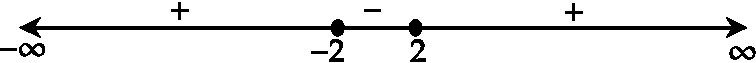
\includegraphics[width=0.55\textwidth]{pset-2 single}
		\end{figure}
		\begin{align*}
		& f^{\prime}(x)>0 \\
		\Rightarrow & \frac{x^{2}-4}{2 x^{2}}>0 \\
		\Rightarrow & x^{2}-4>0 \Rightarrow(x-2)(x+2)>0 \\
		\Rightarrow & x<-2 \quad \text { or } \quad x>2
		\end{align*}
		So, $f(x)$ is increasing on $(-\infty,-2) \cup(2, \infty)$.
	\end{answer}
	\item As $x$ increased from $-\infty$ to $\infty$, the function $f(x)=\frac{e^{x}}{1+e^{x}}$
	(a) monotonically increases
	(b) monotonically decreases
	(c) increases to a maximum value and then decreases
	\begin{tasks}(1)
		\task[\textbf{a.}]Monotonically increases 
		\task[\textbf{b.}]Monotonically decreases
		\task[\textbf{c.}]Increases to a maximum value and then decreases
		\task[\textbf{d.}]Decreases to a minimum value and then increases
	\end{tasks}
	\begin{answer}
		\begin{align*}
		\text{We have,}\\
		f(x)&=\frac{e^{x}}{1+e^{x}}\\
		\text{	Differentiating $f(x)$, we get}\\
		f^{\prime}(x)&=\frac{e^{x}\left(1+e^{x}\right)-e^{2 x}}{\left(1+e^{x}\right)^{2}}\\&=\frac{e^{x}}{\left(1+e^{x}\right)^{2}}
		\end{align*}
		Since $e^{x}$ is positive for all values of $x, f^{\prime}(x)$ is positive for all values of $x$ and hence $f(x)$ monotonically increases. 
		
		
	\end{answer}
	
	\item The Taylor's series expansion of $\frac{\sin x}{x-\pi}$ at $x=\pi$ is given by
	\begin{tasks}(2)
		\task[\textbf{a.}] $1+\frac{(x-\pi)^{2}}{3 !}+\cdots$ 
		\task[\textbf{b.}]$-1-\frac{(x-\pi)^{2}}{3 !}+\cdots$
		\task[\textbf{c.}]$1-\frac{(x-\pi)^{2}}{3 !}+\cdots$ 
		\task[\textbf{d.}]  $-1+\frac{(x-\pi)^{2}}{3 !}+\cdots$
	\end{tasks}
	\begin{answer}
		Taylor's series expansion of $f(x)$ around $x=\pi$ is
		\begin{align*}
		f(x)&=f(\pi)+\frac{x-\pi}{1 !} f^{\prime}(\pi)+\frac{(x-\pi)^{2}}{2 !} f^{\prime \prime}(\pi)+\cdots \\
		\text { Now, } f(\pi)&=\lim _{x \rightarrow \pi} \frac{\sin x}{x-\pi}\\&=\lim _{x \rightarrow \infty} \frac{\cos x}{1}=-1
		\end{align*}
		
		Similarly, by using L'Hospital's rule, we can show that
		\begin{align*}
		f^{\prime}(\pi)&=0\\\text{and} \quad f^{\prime \prime}(\pi)&=-\frac{1}{3}\\
		\text{	So, the expansion is}\quad f(x)&=-1+(-1 / 6)(x-\pi)^{2}+\cdots\\
		f(x)&=-1-\frac{\left(x^{\prime}-\pi\right)^{2}}{3 !}+\cdots
		\end{align*}
		So the correct answer is {\textbf{b}}
	\end{answer}
	
	\item Find $\frac{d z}{d t}$ when $z=x y^{2}+x^{2} y, x=a t^{2}, y=2 a t$
	\begin{answer}
		\begin{align*}
		&\text { We have, } z=x y^{2}+x^{2} y \Rightarrow \frac{\partial z}{\partial x}-y^{2}+2 x y \text { and } \frac{\partial z}{\partial y}=2 x y+x^{2}\\
		&\begin{aligned}
		\text { Also, } x &=a t^{2}, y=2 a t \Rightarrow \frac{d x}{d t}=2 a t, \frac{d y}{d t}=2 a \\
		\text { Hence, }, & \frac{d z}{d t}=\frac{\partial z}{\partial x} \cdot \frac{d x}{d t}+\frac{\partial z}{\partial y} \frac{d y}{d t}=\left(y^{2}+2 x y\right)(2 a t)+\left(2 x y+x^{2}\right) 2 a \\
		&=\left(4 a^{2} t^{2}+2 a t^{2} \cdot 2 a t\right) 2 a t+\left(2 a t^{2} 2 a t+a^{2} t^{4}\right) 2 a \\
		&=8 a^{3} t^{3}+8 a^{3} t^{4}+8 a^{3} t^{3}+2 a^{4} t^{3}\\&=16 a^{3} t^{3}+8 a^{3} t^{4}+2 a^{4} t^{3}\\&=16 a^{3} t^{3}+10 a^{3} t^{4}
		\end{aligned}
		\end{align*}
	\end{answer}
	\item 
	If  $x^{y}+y^{x}=c$,  find the value of $ \frac{d y}{d x}$
	
	
	\begin{answer}
		\begin{align*}
		\text { Let } f(x, y)&=x^{y}+y^{x}\\
		\text { Then, } \frac{\partial f}{\partial x}&=y x^{y-1}+y^{x} \log _{e} y ; \text { Similarly }, \frac{\partial f}{\partial y}=x^{y} \log _{e} x+x y^{x-1}\\
		\therefore \quad \frac{d y}{d x}&=-\frac{\partial f / \partial x}{\partial f / \partial y}=-\frac{y^{x} \log _{e} y+y^{y-1}}{x^{y} \log _{e} x+x y^{x-1}}
		\end{align*}
		
	\end{answer}
	
\end{enumerate}

\newpage
\begin{abox}
	BHU Previous Year Questions
\end{abox}
\section*{\centering{\color{futuringtheme} \underline{Single Variable Calculus}}}

\begin{questions}
	\begin{minipage}{\textwidth}
		\question In the limit $x \rightarrow \infty, \ln (x)-x$
		\exyear{BHU 2012}
	\end{minipage}
	\begin{tasks}(4)
		\task[\textbf{A.}] equals zero
		\task[\textbf{B.}]equals 2
		\task[\textbf{C.}]equals $-\infty$
		\task[\textbf{D.}] equals$+\infty$
	\end{tasks}
	\begin{answer}
		\begin{align*}
		\lim _{x \rightarrow \infty} \ln(x)-x&=-\lim _{x \rightarrow \infty}  (x-\ln (x))\\\
		x-\ln (x) 
		&=\ln \left(e^{x}\right)+\ln \left(x^{-1}\right) \\
		&=\ln \left(\frac{e^{x}}{x}\right)\\\text{But }\lim _{x \rightarrow \infty} \frac{e^{x}}{x}&=\frac{\infty}{\infty}\\
		\intertext{Since the form is indeterminate using L'Hopital's rule we get,}
		\lim _{x \rightarrow \infty} \frac{e^{x}}{x}&=\lim _{x \rightarrow \infty} \frac{e^{x}}{1} \rightarrow \infty\\
		\text{Then,}\ \lim _{x \rightarrow \infty} \ln(x)-x&=-(\lim _{x \rightarrow \infty} \ln(\infty))\\&=-\infty
		\end{align*}
		Correct option is (C)
	\end{answer}
	
	\begin{minipage}{\textwidth}
		\question The mutual potential energy $V$ of two particles depends on their spatial separation as follows $$V=\frac{a}{r^{2}}-\frac{b}{r} ; a>0 ; b>0$$For what separation are the particles in static equilibrium?
		\exyear{BHU 2012}
	\end{minipage}
	\begin{tasks}(4)
		\task[\textbf{A.}] $\frac{a}{b}$
		\task[\textbf{B.}]$\frac{a}{2 b}$
		\task[\textbf{C.}] $\frac{a^{2}}{b}$
		\task[\textbf{D.}] $\frac{2 a}{b}$ 
	\end{tasks}
	\begin{answer}
		At static equilibrium,\begin{align*}
		\frac{\partial v}{\partial r}&=0\\
		\frac{\partial v}{\partial r}&=\frac{\partial( ar^{-2}-br^{-1})}{\partial r }\\
		&=-\frac{2a}{r^{3}}+\frac{b}{r^{2}}\\
		\Rightarrow -\frac{2a}{r^{3}}+\frac{b}{r^{2}}&=0\\
		\frac{2a}{r^{3}}&=\frac{b}{r^{2}}\\
		r&=\frac{2a}{b}
		\end{align*}
		Correct option is (D)
	\end{answer}
	\begin{minipage}{\textwidth}
		\question $\operatorname{Lt}_{x \rightarrow \infty} \sqrt{x}(\sqrt{x+4}-\sqrt{x})$
		\exyear{BHU 2012}
	\end{minipage}
	\begin{tasks}(4)
		\task[\textbf{A.}] 0
		\task[\textbf{B.}]2
		\task[\textbf{C.}] $\frac{1}{2}$
		\task[\textbf{D.}] does not exist
	\end{tasks}
	\begin{answer}
		\begin{align*}
		\lim _{x \rightarrow \infty} \sqrt{x}(\sqrt{x+4}-\sqrt{x})&=\lim _{x \rightarrow \infty} (\sqrt{x^{2}+4x}-{x})\\
		\intertext{Multiply numerator and denominator by the conjugate}
		&=\lim _{x \rightarrow \infty} (\sqrt{x^{2}+4x}-{x})\cdot \frac{(\sqrt{x^{2}+4x}+{x})}{(\sqrt{x^{2}+4x}+{x})}\\
		&=\lim _{x \rightarrow \infty} \frac{x^{2}+4x-x^{2}}{(\sqrt{x^{2}+4x}+{x})}\\
		&=\lim _{x \rightarrow \infty} \frac{4x}{(\sqrt{x^{2}+4x}+{x})}\\
		&=\lim _{x \rightarrow \infty} \frac{4x}{x(\sqrt{1+\frac{4}{x}}+{1})}\\
		&=\lim _{x \rightarrow \infty} \frac{4}{(\sqrt{1+\frac{4}{x}}+{1})} \hspace{2cm} \because \lim _{x \rightarrow \infty}\frac{4}{x}=\frac{4}{\infty}=0 \\
		&=\frac{4}{(\sqrt{1}+{1})}\\
		&=\frac{4}{2}=2
		\end{align*}
		Correct option is(B)
	\end{answer}
	
	\section*{\centering{\color{futuringtheme} \underline{Integral Calculus}}}
	
	\begin{minipage}{\textwidth}
		\question If $[x]$ stands for largest integer not exceeding $x$, then the integral $\int_{-1}^{+2}[x] d x$ equals
		\exyear{BHU 2012}
	\end{minipage}
	
	\begin{tasks}(4)
		\task[\textbf{A.}] 3
		\task[\textbf{B.}]0
		\task[\textbf{C.}]1
		\task[\textbf{D.}] 2
	\end{tasks}
	\begin{answer}
		\begin{align*}
		\int_{-1}^{+2}[x] d x&=\int_{x=-1}^{0}[x] d x+\int_{x=0}^{1}[x] d x+\int_{x=1}^{2}[x] d x \\
		&=\int_{-1}^{0} -1 d x+\int_{0}^{1} 0 d x+\int_{1}^{2} 1 d x\\
		&=\left[-x \right]_{-1} ^{0}+\left[0 \right]_{0} ^{1}+\left[x \right]_{1} ^{2}\\
		&=-1+0+1=0
		\end{align*}
		Correct option is (B)
	\end{answer}
	
	
	\begin{abox}
		HCU Previous Year Questions
	\end{abox}
	\section*{\centering{\color{futuringtheme} \underline{ Serieses}}}
	
	\begin{minipage}{\textwidth}
		\question  The first three terms in the Taylor series expansion of $\sin x$ around $x=\frac{\pi}{2}$ are 
		{\exyear{HCU 2015}}
	\end{minipage}
	\begin{tasks}(2)
		\task[\textbf{A.}]$\left(x-\frac{\pi}{2}\right)-\frac{\left(x-\frac{\pi}{2}\right)^{3}}{3 !}+\frac{\left(x-\frac{\pi}{2}\right)^{5}}{5 !}$ 
		\task[\textbf{B.}]$\left(x-\frac{\pi}{2}\right)+\frac{\left(x-\frac{\pi}{2}\right)^{3}}{3 !}+\frac{\left(x-\frac{\pi}{4}\right)^{5}}{5 !}$ 
		\task[\textbf{C.}] (c) $1-\frac{\left(x-\frac{\pi}{2}\right)^{2}}{2 !}+\frac{\left(x-\frac{\pi}{2}\right)^{4}}{4 !}$
		
		\task[\textbf{D.}]$1+\left(x-\frac{\pi}{2}\right)+\frac{1}{2 !}\left(x-\frac{\pi}{2}\right)^{2}$ 
	\end{tasks}
	\begin{answer}
		\begin{align*}
		f(x)&=\sin x \quad f(\pi / 2)=1\\
		f^{\prime}(x)&=\cos x \quad f^{\prime}(\pi / 2)=0\\
		f^{\prime \prime}(x)&=-\sin x \quad f^{\prime \prime}(\pi / 2)=-1\\
		f^{\prime \prime \prime}(x)&=-\cos x \quad f^{\prime \prime \prime}(\pi / 2)=0 \quad
		\intertext{	Then,  Taylor expansion of $ f(x) $ about $x=\frac{\pi}{2}$}
		f(x)&=f\left(\frac{\pi}{2}\right)+\left(x-\frac{\pi}{2}\right) f^{\prime}\left(\frac{\pi}{2}\right)+\left(x-\frac{\pi}{2}\right)^{2} \frac{f^{\prime \prime}(\pi / 2)}{2 !}+\left(x-\frac{\pi}{2}\right)^{3} \frac{f^{\prime \prime \prime}(\pi / 2)}{3 !}+\cdots\\
		&=1-\left(\frac{x-\frac{\pi}{2}}{2 !}\right)^{2}+\left(\frac{x-\frac{\pi}{4}}{4 !}\right)^{4}-\cdots
		\end{align*}
		
		Correct option is (C)
	\end{answer}
	\begin{minipage}{\textwidth}
		\question The sum of the series
		$$
		1-\frac{1}{3}+\frac{1}{5}-\frac{1}{7}+\frac{1}{9}-\frac{1}{11}+\cdots \cdots
		$$
		is equal to
		{\exyear{HCU 2018}}
	\end{minipage}
	\begin{tasks}(4)
		\task[\textbf{A.}]$\frac{\pi}{2}$. 
		\task[\textbf{B.}]$\frac{\pi}{4}$. 
		\task[\textbf{C.}]$\pi$ 
		\task[\textbf{D.}]$\frac{100}{101}$. 
	\end{tasks}
	\begin{answer}
		\begin{align*}
		\intertext{We know that,}
		\tan ^{-1} x&=x-\frac{x^{3}}{3}+\frac{x^{5}}{5}-\frac{x^{7}}{7}+\ldots \ldots\\ 
		\text{When $x=1$,}\ \tan ^{-1} 1&=1-\frac{1}{3}+\frac{1}{5}-\frac{1}{7}+\frac{1}{9}-\frac{1}{11}+\cdots \cdots\\&=\frac{\pi}{4}
		\end{align*}
		
		Correct option is(B)
	\end{answer}
	\begin{minipage}{\textwidth}
		\question  The product of the two given series
		$$
		\left(x-\frac{1}{3 !} x^{3}+\frac{1}{5 !} x^{5}+\cdots\right)\left(1-\frac{1}{2 !} x^{2}+\frac{1}{4 !} x^{4}+\cdots\right)
		$$
		{\exyear{HCU 2019}}
	\end{minipage}
	\begin{tasks}(4)
		\task[\textbf{A.}] $e^{2 x}$
		\task[\textbf{B.}] $\frac{1}{2}(\cos 2 x)$
		\task[\textbf{C.}] $e^{-2 x}$
		\task[\textbf{D.}] $\frac{1}{2}(\sin 2 x)$
	\end{tasks}
	\begin{answer}
		We know that,
		\begin{align*}
		\sin x&=\left(x-\frac{1}{3 !} x^{3}+\frac{1}{5 !} x^{5}+\cdots\right)\\
		\cos x&=\left(1-\frac{1}{2 !} x^{2}+\frac{1}{4 !} x^{4}+\cdots\right)\\
		\text{Then,}\\
		\sin x \cos x&=\left(x-\frac{1}{3 !} x^{3}+\frac{1}{5 !} x^{5}+\cdots\right)\left(1-\frac{1}{2 !} x^{2}+\frac{1}{4 !} x^{4}+\cdots\right)\\
		\text{But,}\ \sin 2x&=2\sin x \cos x\\\\
		\text{Then,}\\
		\sin x \cos x&=\left(x-\frac{1}{3 !} x^{3}+\frac{1}{5 !} x^{5}+\cdots\right)\left(1-\frac{1}{2 !} x^{2}+\frac{1}{4 !} x^{4}+\cdots\right)=\frac{1}{2}\sin 2x
		\end{align*}
		Correct option is (D)
	\end{answer}
	
	\section*{\centering{\color{futuringtheme} \underline{Trigonometry}}}
	
	\begin{minipage}{\textwidth}
		\question If $\cot \theta=\sin 2 \theta$, the possible values of $\tan \theta$ are
		{\exyear{HCU 2020}}
	\end{minipage}
	\begin{tasks}(4)
		\task[\textbf{A.}]0,1 . 
		\task[\textbf{B.}]$-1,0$. 
		\task[\textbf{C.}]$-1,1$. 
		\task[\textbf{D.}]$-1 / 2,1 / 2$. 
	\end{tasks}
	\begin{answer}
		\begin{align*}
		\cot \theta&=\sin 2 \theta\\
		&=2\sin \theta \cos \theta\\
		\tan \theta &=\frac{1}{\cot \theta}=\frac{1}{2\sin \theta \cos \theta}\\
		\text{Then tan exists only when}\ \sin \theta &= \cos \theta \neq 0\\
		\Rightarrow \theta&= \pm 45^{\circ}
		\text{Then,} \tan \theta &=-1,1
		\end{align*}
		Correct option is(C)
	\end{answer}
	\begin{abox}
		JEST Previous Year Questions
	\end{abox}
	\section*{\centering{\color{futuringtheme} \underline{ Serieses}}}
	
	\begin{minipage}{\textwidth}
		\question As $x \rightarrow 1$, the infinite series $x-\frac{1}{3} x^{3}+\frac{1}{5} x^{5}-\frac{1}{7} x^{7}+\ldots \ldots .$
		\exyear{JEST 2012}
	\end{minipage}
	\begin{tasks}(2)
		\task[\textbf{A.}] diverges
		\task[\textbf{B.}] converges to unity
		\task[\textbf{C.}]converges to $\frac{\pi}{4}$
		\task[\textbf{D.}]none of the above
	\end{tasks}
	\begin{answer}
		\begin{align*}
		\tan ^{-1} x&=x-\frac{x^{3}}{3}+\frac{x^{5}}{5}-\frac{x^{7}}{7}+\ldots \ldots \\ \tan ^{-1} 1&=\frac{\pi}{4}
		\end{align*}
		Correct option is (C)
	\end{answer}
	
	\begin{minipage}{\textwidth}
		\question What is the value of the following series?\\
		$\left(1+\frac{1}{2 !}+\frac{1}{4 !}+\ldots .\right)^{2}-\left(1+\frac{1}{3 !}+\frac{1}{5 !}+\ldots . .\right)^{2}$
		\exyear{JEST 2012}
	\end{minipage}
	\begin{tasks}(4)
		\task[\textbf{A.}] 0
		\task[\textbf{B.}]$e$
		\task[\textbf{C.}]$e^{2}$
		\task[\textbf{D.}]1
	\end{tasks}
	\begin{answer}
		\begin{align*}
		e^{1}&=1+1+\frac{1^{2}}{2 !}+\frac{1^{3}}{3 !}+-; \hspace{0.2cm} e^{-1}=1-1+\frac{1^{2}}{2 !}-\frac{1^{3}}{3 !} \ldots . .\\
		\cosh 1&=\frac{e^{1}+e^{-1}}{2}\\&=1+\frac{1}{2 !}+\frac{1}{4 !}+\ldots\\
		\sinh 1&=\frac{\left(e^{1}-e^{-1}\right)}{2}\\&=1+\frac{1}{3 !}+\frac{1}{5 !}+\ldots\\
		\text{i.e.,}\ \cosh ^{2} 1-\sinh ^{2} 1&=1
		\end{align*}
		Correct option is (D)
	\end{answer}
	
	\begin{minipage}{\textwidth}
		\question What is the value of the following series?
		$$\left(1-\frac{1}{2 !}+\frac{1}{4 !}-\ldots .\right)^{2}+\left(1-\frac{1}{3 !}+\frac{1}{5 !}-\ldots\right)^{2}$$
		\exyear{JEST 2013}
	\end{minipage}
	\begin{tasks}(4)
		\task[\textbf{A.}] 0
		\task[\textbf{B.}]e
		\task[\textbf{C.}]$e^{2}$
		\task[\textbf{D.}]1
	\end{tasks}
	\begin{answer}
		\begin{align*}
		\cos \theta&=1-\frac{\theta^{2}}{2 !}+\frac{\theta^{4}}{4 !} \ldots . \\ \sin \theta&=\theta-\frac{\theta^{3}}{3 !}+\frac{\theta^{5}}{5 !} \ldots . .\\
		\left(1-\frac{1}{2 !}+\frac{1}{4 !} \ldots\right)^{2}+\left(1-\frac{1}{3 !}+\frac{1}{5 !}\right)^{2}&=\cos ^{2} 1+\sin ^{2} 1\\&=1 \hspace{2.5cm}\left[\because \sin ^{2} \theta+\cos ^{2} \theta=1\right]
		\end{align*}
		Correct option is (D)
	\end{answer}
	
	\begin{minipage}{\textwidth}
		\question The sum $\sum_{m=1}^{99} \frac{1}{\sqrt{m+1}+\sqrt{m}}$ is equal to\\
		\exyear{JEST 2015}
	\end{minipage}
	\begin{tasks}(4)
		\task[\textbf{A.}] 9
		\task[\textbf{B.}]$\sqrt{99}-1$
		\task[\textbf{C.}]$\frac{1}{(\sqrt{99}-1)}$
		\task[\textbf{D.}]11
	\end{tasks}
	\begin{answer}
		\begin{align*}
		\sum_{m=1}^{99} \frac{1}{\sqrt{m+1}+\sqrt{m}}&=\sum_{m=1}^{99} \frac{\sqrt{m+1}-\sqrt{m}}{(m+1)-m}\\&=\sum_{m=1}^{99} \sqrt{m+1}-\sqrt{m}\\
		&=\sqrt{2}-\sqrt{1}+\sqrt{3}-\sqrt{2} \ldots . .+\sqrt{100}-\sqrt{99}\\&=\sqrt{100}-\sqrt{1}\\&=10-1=9
		\end{align*}
		Correct option is (A)
	\end{answer}
	
	\begin{minipage}{\textwidth}
		\question The sum of the infinite series $1-\frac{1}{3}+\frac{1}{5}-\frac{1}{7}+\ldots$ is
		\exyear{JEST 2016}
	\end{minipage}
	\begin{tasks}(4)
		\task[\textbf{A.}] $2 \pi$
		\task[\textbf{B.}]$\pi$
		\task[\textbf{C.}]$\frac{\pi}{2}$
		\task[\textbf{D.}]$\frac{\pi}{4}$
	\end{tasks}
	\begin{answer}
		\begin{align*}
		\intertext{The series expansion of  $ \tan ^{-1} x  $  in interval $ -1<x \leq 1 $ is,}
		\tan ^{-1} x&=x-\frac{1}{3} x^{3}+\frac{1}{5} x^{5}-\frac{1}{7} x^{7}+\cdots
		\intertext{Putting $ x=1, $ we get,}
		\tan ^{-1} 1&=1-\frac{1}{3}+\frac{1}{5}-\frac{1}{7}+\cdots \cdot \\&=1-\frac{1}{3}+\frac{1}{5}-\frac{1}{7} \cdots \cdot\\&=\frac{\pi}{4}
		\end{align*}
		Correct option is (D)
	\end{answer}
	\section*{\centering{\color{futuringtheme} \underline{Integral Calculus}}}
	
	\begin{minipage}{\textwidth}
		\question If $[\mathrm{x}]$ denotes the greatest integer not exceeding $\mathrm{x}$, then $\int_{0}^{\infty}[x] e^{-x} d x$
		\exyear{JEST 2012}
	\end{minipage}
	\begin{tasks}(4)
		\task[\textbf{A.}] $\frac{1}{e-1}$
		\task[\textbf{B.}]1
		\task[\textbf{C.}]$\frac{e-1}{e}$
		\task[\textbf{D.}]$\frac{e}{e^{2}-1}$
	\end{tasks}
	\begin{answer}
		\begin{align*}
		[x]=0 \rightarrow 0 \leq x<1&;\hspace{0.2cm} [x]=1\rightarrow 1 \leq x<2; \hspace{0.2cm} [x]=2 \rightarrow 2 \leq x<3\\
		\intertext{Then,}\int_{0}^{\infty}[x] e^{-x} d x&=\int_{0}^{1}[x] e^{-x} d x+\int_{1}^{2}[x] e^{-x} d x+\int_{2}^{3}[x] e^{-x} d x+\int_{3}^{4}[x] e^{-x} d x\\
		&\Rightarrow 0+\int_{1}^{2} 1 . e^{-x} d x+\int_{2}^{3} 2 . e^{-x} d x+\int_{3}^{4} 3 \cdot e^{-x} d x\\&=\left[-e^{-x}\right]_{1}^{2}+2\left(-e^{-x}\right)_{2}^{3}+3\left(-e^{-x}\right)_{3}^{4}+\ldots\\
		&=e^{-1}-e^{-2}+2 e^{-2}-2 e^{-3}+3 e^{-3}-3 e^{-4}+4 e^{-4}-4 e^{-5}+\\
		&=e^{-1}+e^{-2}+e^{-3}+e^{-4}+\ldots \ldots \infty\\
		&=\frac{e^{-1}}{1-e^{-1}}=\frac{1}{e-1}\hspace{2cm}\left(\because r=\frac{e^{-2}}{e^{-1}}=e^{-2+1}=e^{-1}\right)
		\end{align*}
		Correct option is (A)
	\end{answer}
	\section*{\centering{\color{futuringtheme} \underline{Trigonometry}}}
	
	
	\begin{minipage}{\textwidth}
		\question A semicircular piece of paper is folded to make a cone with the centre of the semicircle as the apex. The half-angle of the resulting cone would be:
		\exyear{JEST 2016}
	\end{minipage}
	\begin{tasks}(4)
		\task[\textbf{A.}] $90^{\circ}$
		\task[\textbf{B.}]$60^{\circ}$
		\task[\textbf{C.}]$45^{\circ}$
		\task[\textbf{D.}]$30^{\circ}$
	\end{tasks}
	\begin{answer}
		When the semicircular piece of paper is folded to make a cone, the circumference ofbase is equal to the circumference of the original semicircle. Let $r$ be the radius of the base of the cone and $R$ be the radius of the semicircle.
		\begin{align*}
		\text{Hence,}\ 2 \pi r&=\pi R \Rightarrow r=\frac{R}{2}
		\intertext{The stay height of the come will also be R.}
		\text{Hence,}\ \sin \alpha&=\frac{R / 2}{R}=\frac{1}{2}\\
		\text{Thus, }\ \alpha&=30^{\circ}
		\end{align*}
		\begin{figure}[H]
			\begin{center}
				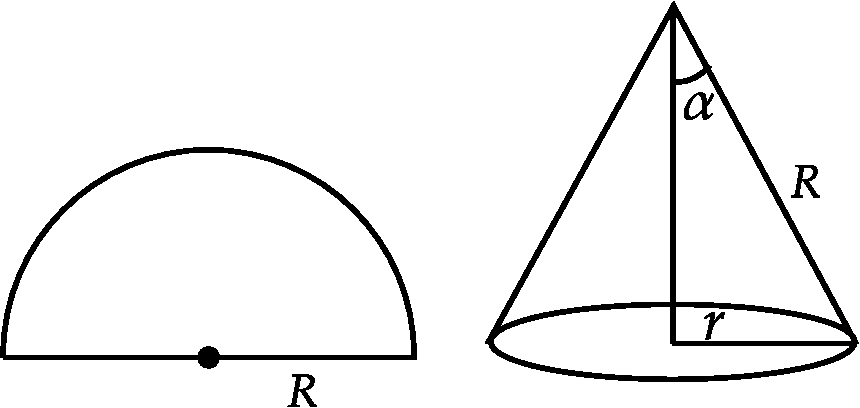
\includegraphics[width=4.5cm,height=2.5cm]{32-S-crop}
			\end{center}
		\end{figure}
		Correct option is (D)
	\end{answer}
	
\end{questions}




